% pdflatex -shell-escape software-analysis-main.tex
\documentclass[12pt,openany]{book}

\usepackage{kotex}
\usepackage{commath}
\usepackage{slantsc}
\usepackage{hyperref}
\usepackage{stmaryrd} %llbracket
\usepackage{adjustbox}
\usepackage{enumerate}

\usepackage{cite}
\usepackage[numbers]{natbib}
\usepackage{amsthm}

% Define custom theorem styles
\newtheoremstyle{dotless} % Name of the style
{3pt} % Space above
{3pt} % Space below
{\itshape} % Body font
{} % Indent amount
{\bfseries} % Theorem head font
{} % Punctuation after theorem head
{2.5mm} % Space after theorem head
{} % Theorem head spec

\newtheoremstyle{definitionstyle} % Name of the style
{3pt} % Space above
{3pt} % Space below
{} % Body font
{} % Indent amount
{\bfseries} % Theorem head font
{.} % Punctuation after theorem head
{2.5mm} % Space after theorem head
{} % Theorem head spec

% Applying custom styles
\theoremstyle{dotless}
\newtheorem{proposition}{Proposition}[section] % Theorem environment with section-wise numbering
\newtheorem{theorem}{Theorem}[section] % Theorem environment with section-wise numbering
\newtheorem{lemma}[theorem]{Lemma} % Lemma shares the counter with theorem
\newtheorem{corollary}[theorem]{Corollary} % Corollary shares the counter with theorem

\theoremstyle{definitionstyle}
\newtheorem{definition}{Definition}[section] % Definition shares the counter with theorem
\newtheorem{example}{Example}[section] % Example shares the counter with theorem
\newtheorem{exercise}{Exercise}[section] % Example shares the counter with theorem
\newtheorem{remark}{Remark}[section] % Remark shares the counter with theorem
\newtheorem*{note}{Note}

% Colors
\usepackage[dvipsnames,table]{xcolor}
\definecolor{titleblue}{RGB}{0,53,128}
\definecolor{chaptergray}{RGB}{140,140,140}
\definecolor{sectiongray}{RGB}{180,180,180}

\definecolor{thmcolor}{RGB}{231, 76, 60}
\definecolor{defcolor}{RGB}{52, 152, 219}
\definecolor{lemcolor}{RGB}{155, 89, 182}
\definecolor{corcolor}{RGB}{46, 204, 113}
\definecolor{procolor}{RGB}{241, 196, 15}
\definecolor{execolor}{RGB}{90, 128, 127}

% Fonts
\usepackage[T1]{fontenc}
\usepackage[utf8]{inputenc}
\usepackage{newpxtext,newpxmath}
\usepackage{sectsty}
\allsectionsfont{\sffamily\color{titleblue}\mdseries}

% Page layout
\usepackage{geometry}
\geometry{a4paper,left=.8in,right=.6in,top=.75in,bottom=1in,heightrounded}
\usepackage{fancyhdr}
\fancyhf{}
\fancyhead[LE,RO]{\thepage}
\fancyhead[LO]{\nouppercase{\rightmark}}
\fancyhead[RE]{\nouppercase{\leftmark}}
\renewcommand{\headrulewidth}{0.5pt}
\renewcommand{\footrulewidth}{0pt}

% Chapter formatting
\usepackage{titlesec}
\titleformat{\chapter}[display]
{\normalfont\sffamily\Huge\bfseries\color{titleblue}}{\chaptertitlename\ \thechapter}{20pt}{\Huge}
\titleformat{\section}
{\normalfont\sffamily\Large\bfseries\color{titleblue!100!gray}}{\thesection}{1em}{}
\titleformat{\subsection}
{\normalfont\sffamily\large\bfseries\color{titleblue!75!gray}}{\thesubsection}{1em}{}

% Table of contents formatting
\usepackage{tocloft}
\renewcommand{\cftchapfont}{\sffamily\color{titleblue}\bfseries}
\renewcommand{\cftsecfont}{\sffamily\color{titleblue!100!gray}}
\renewcommand{\cftsubsecfont}{\sffamily\color{titleblue!75!gray}}
\renewcommand{\cftchapleader}{\cftdotfill{\cftdotsep}}

\usepackage{tcolorbox}
\tcbset{colback=white, arc=5pt}

\definecolor{defcolor}{RGB}{52, 152, 219}
\definecolor{procolor}{RGB}{241, 196, 15}
\definecolor{thmcolor}{RGB}{231, 76, 60}
\definecolor{lemcolor}{RGB}{155, 89, 182}
\definecolor{corcolor}{RGB}{46, 204, 113}
\definecolor{execolor}{RGB}{90, 128, 127}

% Define a new command for the custom tcolorbox
\newcommand{\defbox}[2][]{%
	\begin{tcolorbox}[colframe=defcolor, title={\color{white}\bfseries #1}]
		#2
	\end{tcolorbox}
}

\newcommand{\probox}[2][]{%
	\begin{tcolorbox}[colframe=procolor, title={\color{white}\bfseries #1}]
		#2
	\end{tcolorbox}
}

\newcommand{\thmbox}[2][]{%
	\begin{tcolorbox}[colframe=thmcolor, title={\color{white}\bfseries #1}]
		#2
	\end{tcolorbox}
}

\newcommand{\corbox}[2][]{%
	\begin{tcolorbox}[colframe=corcolor, title={\color{white}\bfseries #1}]
		#2
	\end{tcolorbox}
}
\usepackage{tikz}
\usepackage{tikz-cd}
\usetikzlibrary{shadows}
\usetikzlibrary{shapes.geometric, arrows.meta, positioning}
\usepackage[ruled,linesnumbered]{algorithm2e}
\usepackage{setspace}
\usepackage{algpseudocode}
\SetKwComment{Comment}{/* }{ */}
\SetKw{Break}{break}
\SetKw{Downto}{downto}
\SetKwProg{Fn}{Function}{:}{end}
\SetKwProg{Procedure}{procedure}{:}{end}
\SetKwProg{Construct}{Construct}{:}{end}
\SetKwFunction{KeyGen}{KeyGen}

%Listing
\usepackage{listings} %Code
\renewcommand{\lstlistingname}{Code}%
\definecolor{keyword}{RGB}{255, 0, 0}
\definecolor{identifier}{RGB}{0, 0, 255}
\definecolor{comment}{RGB}{0, 128, 0}
\definecolor{string}{RGB}{163, 21, 21}

\lstdefinestyle{c}{
	language=C,
	basicstyle=\ttfamily\small,
	keywordstyle=\color{keyword},
	identifierstyle=\color{identifier},
	commentstyle=\color{comment}\itshape,
	stringstyle=\color{string},
	showstringspaces=false,
	%	numberstyle=\tiny\color{gray},
	%	numbersep=5pt,
	frame=single,
	tabsize=4,
	captionpos=b,
	breaklines=true,
	breakatwhitespace=true,
	%	numbers=left
}
\newcommand{\A}{\mathbb{A}}
\newcommand{\B}{\mathbb{B}}
\newcommand{\C}{\mathbb{C}}
\newcommand{\F}{\mathbb{F}}
\newcommand{\N}{\mathbb{N}}
\newcommand{\Q}{\mathbb{Q}}
\newcommand{\R}{\mathbb{R}}
\newcommand{\Z}{\mathbb{Z}}

\newcommand{\cP}{\mathcal{P}}
\newcommand{\cR}{\mathcal{R}}

\newcommand{\pl}{\textsf{PL}\ }
\newcommand{\fol}{\textsf{FOL}\ }
\newcommand{\hol}{\textsf{HOL}\ }

\newcommand{\oracle}{\textsc{Oracle}}
\newcommand{\sub}[1]{\textsf{sub}\left(#1\right)}

\newcommand{\dom}{\mathsf{dom}}
\newcommand{\cdm}{\mathsf{cdm}}
\newcommand{\range}{\mathsf{range}}

\newcommand{\free}{\mathsf{free}}
\newcommand{\bound}{\mathsf{bound}}

\newcommand{\true}{\textcolor{red}{\texttt 1}}
\newcommand{\false}{\textcolor{red}{\texttt 0}}
\newcommand{\id}{\textnormal{id}}

\newcommand{\sol}{\textcolor{magenta}{\bf Sol}}
\newcommand{\ie}{i.\,e.}
\newcommand{\eg}{e.\,g.}
\newcommand{\wrt}{w.\,r.\,t.\ }
\newcommand{\aka}{a.\,k.\,a.\ }
\newcommand{\cf}{cf.\ }
\newcommand{\etc}{etc.\ }
%\input{cryptanalysis-lstlisting}
%\usepackage[backend=biber,style=numeric,citestyle=numeric]{biblatex}
%\addbibresource{sv-references.bib}
\begin{document}
	
	\begin{titlepage}
    \centering
    
    \vspace*{1cm}
    
    \Huge\textsf{\textbf{Software Verification}}
    
    \vspace{0.5cm}
%   \LARGE\textsf{- A Deep Dive into Testing and Validation -}
    \LARGE\textsf{- Logic-based Program Verification -}
    
    \vspace{1.5cm}
    \textbf{Ji, Yong-Hyeon}

	\vspace{2cm}
%	\begin{figure}[h!]\centering
%	\begin{tikzpicture}
%		% Set colors for different logics
%		\definecolor{plcolor}{RGB}{255, 204, 204}
%		\definecolor{folcolor}{RGB}{204, 229, 255}
%		\definecolor{holcolor}{RGB}{204, 255, 204}
%		
%		% Draw the Higher-Order Logic (HOL) circle
%		\fill[holcolor] (0,0) circle (6cm);
%		\draw (0,0) circle (6cm);
%		\node at (0, 5.25) {\bf Higher-Order Logic (HOL)};
%		
%		% Draw the First-Order Logic (FOL) circle
%		\fill[folcolor] (0,0) circle (5cm);
%		\draw (0,0) circle (5cm);
%		\node at (0, 3.75) {\bf First-Order Logic (FOL)};
%		
%		% Draw the Propositional Logic (PL) circle
%		\fill[plcolor] (0,0) circle (3cm);
%		\draw (0,0) circle (3cm);
%		\node at (0, 0) {\bf Propositional Logic (PL)};
%		
%	\end{tikzpicture}
%	\end{figure}
	\begin{center}
	\adjustbox{scale=.9}{
	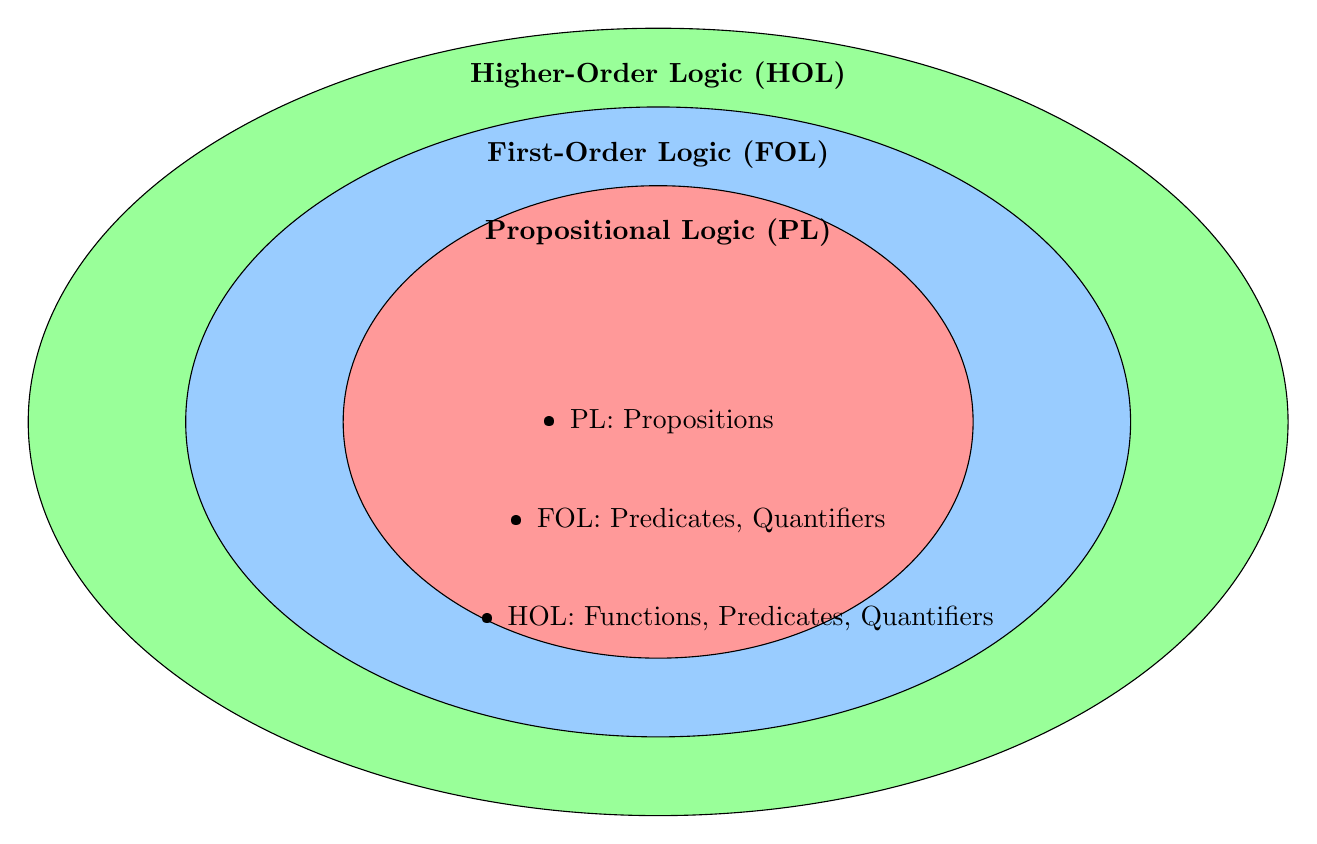
\begin{tikzpicture}
		
		% Define colors
		\definecolor{plcolor}{RGB}{255, 153, 153}
		\definecolor{folcolor}{RGB}{153, 204, 255}
		\definecolor{holcolor}{RGB}{153, 255, 153}
		
		% Draw the Higher-Order Logic (HOL) ellipse
		\fill[holcolor, draw=black] (0,0) ellipse (8cm and 5cm);
		\node at (0, 4.4) {\textbf{Higher-Order Logic (HOL)}};
		
		% Draw the First-Order Logic (FOL) ellipse
		\fill[folcolor, draw=black] (0,0) ellipse (6cm and 4cm);
		\node at (0, 3.4) {\textbf{First-Order Logic (FOL)}};
		
		% Draw the Propositional Logic (PL) ellipse
		\fill[plcolor=, draw=black] (0,0) ellipse (4cm and 3cm);
		\node at (0, 2.4) {\textbf{Propositional Logic (PL)}};
		
		% Add arrows to show inclusion
%		\draw[thick,-Stealth] (0,0) -- (.5,-1.25) node[midway,above] {\footnotesize More expressive};
%		\draw[thick,->] (2,1.2) -- (2.7,1.5);
%		\draw[thick,->] (1.5,-1.2) -- (2.3,-1.5);
		
		% Add dimensions
		\node at (1,-2.5) {\textbullet \, HOL: Functions, Predicates, Quantifiers};
		\node at (.5,-1.25) {\textbullet \, FOL: Predicates, Quantifiers};
		\node at (0,0) {\textbullet \, PL: Propositions};
	\end{tikzpicture}}
\end{center}
	
	\vspace{1.5cm}
    \vfill
    A document presented for\\
    the Software Verification
    
    \vspace{0.8cm}
    {\large\textsf{Department of Information Security, Cryptology, and Mathematics}\par}
    {\large\textsf{College of Science and Technology}\par}
    {\large\textsf{Kookmin University}\par}
    \vspace{.25in}
    {\large \textsf{\today}\par}
    
%    \Large{Institution Name}\\
%    Date
\end{titlepage}


	\tableofcontents
	\newpage
	\section*{Symbols}
In this paper, symbols are defined as follows. \\ \ \\ 
$
\begin{array}{cl}
	I\models P & \text{$I$ satisfies $P$} \\
	I\not\models P & \text{$I$ does not satisfies $P$} \\
\end{array}
$
	\newpage
	\chapter{Introduction}
	% Chapter I. Introduction

\cite{youtube:COSE419-Lecture1-1}
\cite{youtube:COSE419-Lecture1-2}
\cite{naver:bycho211-1}
	
	\newpage
%	\chapter{Greybox Fuzzing and Concolic Testing}
%	% Propositional Logic I

References:\cite{youtube:COSE419-Lecture4-1}

Propositional logic is a branch of logic that deals with propositions which can be either true or false. The basic components and operations in propositional logic are as follows:

%\begin{align*}
%	\texttt{<atom>} ::= &\ \text{"P"}\ |\ \text{"Q"}\ |\ \text{"R"}\ |\ \ldots\
%\end{align*}
%
%\begin{align*}
%	\texttt{<literal>} ::= &\ \texttt{<atom>} \\
%	&\ |\ \text{"¬"}\ \texttt{<atom>}
%\end{align*}
%
%\begin{align*}
%	\texttt{<formula>} ::= &\ \texttt{<literal>} \\
%	&\ |\ \text{"("}\ \texttt{<formula>}\ \text{")"} \\
%	&\ |\ \text{"¬"}\ \texttt{<formula>} \\
%	&\ |\ \text{"("}\ \texttt{<formula>}\ \text{"∧"}\ \texttt{<formula>}\ \text{")"} \\
%	&\ |\ \text{"("}\ \texttt{<formula>}\ \text{"∨"}\ \texttt{<formula>}\ \text{")"} \\
%	&\ |\ \text{"("}\ \texttt{<formula>}\ \text{"→"}\ \texttt{<formula>}\ \text{")"} \\
%	&\ |\ \text{"("}\ \texttt{<formula>}\ \text{"↔"}\ \texttt{<formula>}\ \text{")"} \\
%\end{align*}

\section{Syntax and Semantic of Propositional Logic}
\begin{center}
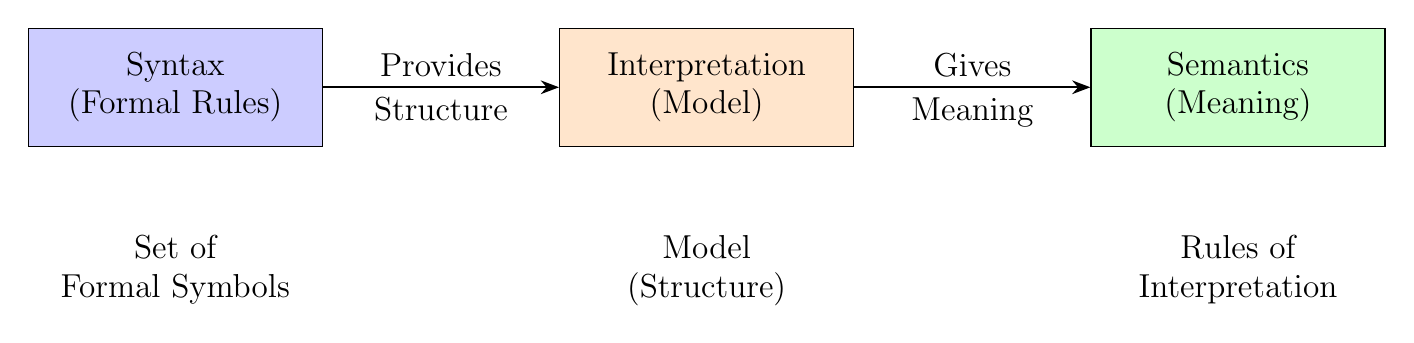
\begin{tikzpicture}[
	every node/.style={font=\large, node distance=3cm},
	process/.style={rectangle, draw, text width=3.5cm, align=center, minimum height=1.5cm},
	arrow/.style={thick, ->, >=Stealth}
	]
	
	% Nodes
	\node[process, fill=blue!20] (syntax) {Syntax \\ (Formal Rules)};
	\node[process, fill=orange!20, right=of syntax] (interpretation) {Interpretation \\ (Model)};
	\node[process, fill=green!20, right=of interpretation] (semantics) {Semantics \\ (Meaning)};
	
	% Arrows
	\draw[arrow] (syntax) -- node[above, align=center] {Provides} node[below, align=center] {Structure} (interpretation);
	\draw[arrow] (interpretation) -- node[above, align=center] {Gives} node[below, align=center] {Meaning} (semantics);
	
	% Labels
	\node[below=1cm of syntax, align=center] {Set of \\ Formal Symbols};
	\node[below=1cm of interpretation, align=center] {Model \\ (Structure)};
	\node[below=1cm of semantics, align=center] {Rules of \\ Interpretation};
\end{tikzpicture}
\end{center}
\subsection{Syntax}
% Tree illustrating Atoms, Literals, and Formulas
\begin{center}\adjustbox{scale=.75}{
%\begin{tikzpicture}[
%	level distance=2.5cm,
%	sibling distance=3.5cm,
%	every node/.style={draw, shape=rectangle, rounded corners, align=center}
%	]
%	
%	% Root
%	\node {Boolean Logic}
%	% Level 1
%	child {node {Unary}
%	}
%	child {node {Binary}
%	}
%	% Level 2
%	child {node {Atom}
%		% Level 3 for Unary
%		child {node {Unary: $\bot$ (false)}}
%		child {node {Unary: $\top$ (true)}}
%		% Level 3 for Binary
%		child {node {Binary: $P, Q, R, \dots$}}
%	}
%	child {node {Literal}
%		% Level 3 for Unary
%		child {node {Unary: $\neg \bot$}}
%		child {node {Unary: $\neg \top$}}
%		% Level 3 for Binary
%		child {node {Binary: $\neg P, \neg Q, \neg R, \dots$}}
%	}
%	child {node {Formula}
%		% Level 3 for Unary
%		child {node {Unary: $\neg F$ (not)}}
%		% Level 3 for Binary
%		child {node {Binary: $F_1 \land F_2$ (and)}}
%		child {node {Binary: $F_1 \lor F_2$ (or)}}
%		child {node {Binary: $F_1 \to F_2$ (implies)}}
%		child {node {Binary: $F_1 \leftrightarrow F_2$ (if and only if)}}
%	};
%	
%\end{tikzpicture}
}
\end{center}
%\begin{tikzpicture}[
%	node distance=2cm,
%	every node/.style={draw, rectangle, rounded corners, align=center},
%	level 1/.style={sibling distance=6cm},
%	level 2/.style={sibling distance=3cm},
%	level 3/.style={sibling distance=2cm}
%	]
%	
%	% Root node
%	\node (formula) {Formula};
%	
%	% Level 1
%	\node [below left=of formula] (literal) {Literal}
%	child {node (atom) {Atom\\(e.g., $P, Q$)}}
%	child {node (negatom) {Negation of Atom\\(e.g., $\lnot P, \lnot Q$)}};
%	
%	\node [below right=of formula] (special) {Special Constant}
%	child {node {True\\($\top$)}}
%	child {node {False\\($\bot$)}};
%	
%	% Connections from Formula to Literals and Special Constants
%	\draw (formula) -- (literal);
%	\draw (formula) -- (special);
%	
%	% Level 2
%	\node [below=2cm of literal] (unary) {Unary Truth Function}
%	child {node (neg) {Negation\\($\lnot F$)}};
%	
%	\node [below=2cm of special] (binary) {Binary Truth Function}
%	child {node (and) {Conjunction\\($F_1 \land F_2$)}}
%	child {node (or) {Disjunction\\($F_1 \lor F_2$)}}
%	child {node (imp) {Implication\\($F_1 \to F_2$)}}
%	child {node (bicond) {Biconditional\\($F_1 \leftrightarrow F_2$)}};
%	
%	% Connections from Literals to Unary Truth Function
%	\draw (literal) -- (unary);
%	
%	% Connections from Special Constants to Binary Truth Function
%	\draw (special) -- (binary);
%	
%	% Level 3 Connections from Unary and Binary Truth Functions to Formulas
%	\foreach \child in {neg, and, or, imp, bicond}
%	\draw (\child) -- ++(0,-1) node[draw, rectangle, rounded corners, align=center] {Formula};
%	
%	% Additional connections to demonstrate usage
%	\draw (negatom) -- (neg);
%	\draw (atom) -- (unary);
%	\draw (negatom) -- (unary);
%	
%\end{tikzpicture}
\begin{itemize}
	\item \textbf{Atom}: basic elements
	\begin{itemize}
		\item truth symbols $\bot$(``false'') and $\top$(``true'')
		\item propositional variables $P,Q,R,\dots$
	\end{itemize}
	\item \textbf{Literal}: an atom $\alpha$ or its negation $\lnot\alpha$.
	\item \textbf{Formula}: a literal or the application of a logical connective (boolean connectives) to formulas
	\[
	\begin{array}{ccll}
		F & \to & \bot \\
		& | & \top \\
		& | & P \\
		& | & \lnot F & \text{negation (``not'')} \\
		& | & F_1\land F_2 & \text{conjunction (``and'')} \\
		& | & F_1\lor F_2 & \text{disjunction (``or'')} \\
		& | & F_1\to F_2 & \text{implication (``implies'')} \\
		& | & F_1\leftrightarrow F_2 & \text{iff (``if and only if'')}
	\end{array}
	\]
	\item[]
	\item Formula $G$ is a \textbf{subformula} of formula $F$ if it occurs syntactically within $G$.
	\begin{align*}
		\sub{\bot} &= \set{\bot} \\
		\sub{\top} &= \set{\top} \\
		\sub{P} &= \set{P} \\
		\sub{\lnot F} &= \set{\lnot F}\cup\sub{F} \\
		\sub{F_1\land F_2} &= \set{F_1\land F_2}\cup\sub{F_1}\cup\sub{F_2}
		&\vdots
	\end{align*}
	\item Consider $F:(P\land Q)\to (P\lor\lnot Q)$. Then \[
	\sub{F}=\set{F,P\land Q,P\lor\lnot Q,P,Q,\lnot Q}.
	\]
	\begin{center}\begin{minipage}{.45\textwidth}\centering\adjustbox{scale=.8}{
%\begin{tikzpicture}[
%%	sibling distance=8cm,
%%	level distance=2cm,
%	every node/.style = {shape=rectangle, rounded corners, draw, align=center},
%	level 1/.style = {sibling distance=2cm, level distance=1cm},
%	level 2/.style = {sibling distance=1cm, level distance=1cm},
%	level 3/.style = {sibling distance=1cm, level distance=1cm}
%%	edge from parent/.style = {draw, -{Latex}, thick},
%%	edge from parent path = {(\tikzparentnode.south) -- ++(0,-1.5em) -| (\tikzchildnode.north)}
%	]
%	\node {$(P\land Q)\to(P\lor\lnot Q)$}
%	child { node {$P\land Q$}
%		child { node {$P$} }
%		child { node {$Q$} }
%	}
%	child { node {$P\lor\lnot Q$}
%		child { node {$P$}
%		}
%		child { node {$\lnot Q$} 
%			child { node {$Q$} } 
%		}
%	};
%\end{tikzpicture}
\begin{tikzcd}
	& (P\land Q)\to(P\lor\lnot Q) \arrow[ld, no head] \arrow[rd, no head] &                                                      \\
	P\land Q \arrow[dd, no head] \arrow[rdd, no head] &                                                                     & P\lor\lnot Q \arrow[d, no head] \arrow[ldd, no head] \\
	&                                                                     & \lnot Q                                              \\
	Q                                                 & P                                                                   &          
\end{tikzcd}
}
\end{minipage}
\begin{minipage}{.45\textwidth}\centering\adjustbox{scale=.8}{
\begin{tikzcd}
	P \arrow[ddd, no head] \arrow[rrddd, no head] &                          & Q \arrow[d, no head] \arrow[llddd, no head] \\
	&                          & \lnot Q \arrow[dd, no head]                 \\
	&                          &                                             \\
	P\land Q \arrow[rdd, no head]                 &                          & P\lor\lnot Q \arrow[ldd, no head]           \\
	&                          &                                             \\
	& P\land Q\to P\lor\lnot Q &                                            
\end{tikzcd}}
\end{minipage}	
%\begin{minipage}{.48\textwidth}\adjustbox{scale=.5}{
%		\begin{tikzpicture}[
%			edge from parent/.style={draw, -latex},
%			sibling distance=4cm,
%			level distance=2cm,
%			every node/.style={draw, shape=rectangle, rounded corners, align=center}
%			]
%			
%			% Unary and Binary Nodes
%			\node {Boolean Logic}
%			child {node {Unary}
%				child {node {Atom}}
%				child {node {Literal}}
%				child {node {Formula}}
%			}
%			child {node {Binary}
%				child {node {Atom}}
%				child {node {Literal}}
%				child {node {Formula}}
%			};
%			
%			% Atom, Literal, and Formula Nodes
%			\node (atom) [below=4cm of Boolean-1-1] {Atom}
%			child {node {$\bot$}}
%			child {node {$\top$}};
%			\node (literal) [below=4cm of Boolean-1-2] {Literal}
%			child {node {$\neg \alpha$}};
%			\node (formula) [below=4cm of Boolean-1-3] {Formula}
%			child {node {$F$}}
%			child {node {$\neg F$}};
%			
%			% Connections to common nodes
%			\draw[-] (Boolean-1-1) -- (atom);
%			\draw[-] (Boolean-2-1) -- (atom);
%			\draw[-] (Boolean-1-2) -- (literal);
%			\draw[-] (Boolean-2-2) -- (literal);
%			\draw[-] (Boolean-1-3) -- (formula);
%			\draw[-] (Boolean-2-3) -- (formula);
%	\end{tikzpicture}
%\end{minipage}
\end{center}
	\item The strict subformulas of a formula are all its subformulas except itself.
	\item[]
	\item To minimally use parentheses, we define the relative precedence of the logical connectives from highest to lowest as follows: \[
	\lnot\quad\land\quad\lor\quad\rightarrow\quad\leftrightarrow
	\]
	\item (Currying) Additionally, $\rightarrow$ and $\leftrightarrow$ associate to the right, e.g., \[
	P\to Q\to R\iff P\to(Q\to R).
	\]
	\item Example:
	\begin{itemize}
		\item $(P\land Q)\to (P\lor\lnot Q)\iff P\land Q\to P\lor \lnot Q$
		\item $(P_1\land((\lnot P_2)\land\top))\lor((\lnot P_1)\land P_2)\iff P_1\land P_2\top\lor\lnot P_1\land P_2$
	\end{itemize}
\end{itemize}

\subsection{Semantics}
\begin{itemize}
	\item The semantics of a logic provides its meaning. The meaning of a PL formula is either true or false.
	\item The semantics of a formula is defined with an \textbf{interpretation} (or assignment) that assigns truth values to propositional variables.
	\item For example, $F:P\land Q\to P\lor\land Q$ evaluates to true under the interpretation $I:\set{P\mapsto \text{true},Q\mapsto\text{false}}:$
	\begin{table}[h!]\centering\setstretch{1.25}
		\begin{tabular}{c|c||c|c|c|c}
			\hline
			$P$ & $Q$ & $\lnot Q$ & $P\land Q$ & $P\lor \lnot Q$ & $F$ \\ \hline
			1 & 0 & 1 & 0 & 1 & 1 \\ \hline
		\end{tabular}
	\end{table}
	\item The tabular notation is unsuitable for predicate logic. Instead, we define the semantics inductively.
\end{itemize}

\subsection{Inductive Definition of Semantics}
In an inductive definition, the meaning of basic elements is defined first.
The meaning of complex elements is defined in terms of subcomponents.
\begin{itemize}
	\item We write $I\models F$ if $F$ evaluates to \textbf{true} under $I$.
	\item We write $I\not\models F$ if $F$ evaluates to \textbf{false} under $I$.
\end{itemize}
Note that \[
\begin{array}{ll}
I\models \top,\quad I\not\models\bot, & \\
I\models P &\text{iff}\ I[P]=\text{true} \\
I\models \lnot F &\text{iff}\ I[P]=\text{false} \\
I\models\lnot F &\text{iff}\ I\not\models F \\
I\models F_1\land F_2 &\text{iff}\ I\models F_1\ \text{and}\ I\models F_2 \\
I\models F_1\lor F_2 &\text{iff}\ I\models F_1\ \text{or}\ I\models F_2 \\
I\models F_1\to F_2 &\text{iff}\ I\not\models F_1\ \text{or}\ I\models F_2 \\
I\models F_1\leftrightarrow F_2 &\text{iff}\ (I\models F_1\ \text{and}\ I\models F_2)\ \text{or}\ (I\not\models F_1\ \text{and}\ I\not\models F_2)
\end{array}
\]
\vspace{12pt}
\begin{example}
	Consider the formula \[
	F:P\land Q\to P\lor\lnot Q
	\] and the interpretation \[
	I:\set{P\mapsto\text{true},Q\mapsto\text{false}}.
	\] The truth value of $F$ is computed as follows: \[
	\begin{array}{ll}
		1.\quad I\models P &\text{since $I[P]=\text{true}$} \\
		2.\quad I\not\models Q &\text{since $I[P]=\text{true}$} \\
		3.\quad I\models \lnot Q &\text{by 2 and semantics of $\lnot$} \\
		4.\quad I\not\models P\land Q &\text{by 2 and semantics of $\land$} \\
		5.\quad I\models P\lor \lnot Q &\text{by 1 and semantics of $\lor$} \\
		6.\quad I\models F &\text{by 4 and semantics of $\to$} \\
	\end{array}
	\]
\end{example}

\section{Satisfiability and Validity}
\begin{itemize}
	\item A formula $F$ is \textbf{satisfiable} iff there exists an interpretation $I$ such that $I\models F$.
	\item A formula $F$ is \textbf{valid} iff for all interpretations $I$, $I\models F$.
	\item Satisfiability and validity are dual: \[
	\text{$F$ is valid}\iff\text{$\lnot F$ is unsatisfiable}
	\]
	\begin{proof}
		content...
	\end{proof}
	\item We can check satisfiability by deciding validity, and vice versa.
\end{itemize}

\begin{figure}[h!]\centering
\begin{tikzcd}
	& \text{VALID} \arrow[dr, "\neg"] & \\
	\text{SAT} \arrow[ur, "\neg"] \arrow[rr, "\neg"] & & \text{UNSAT} \\
	& \text{INVALID} \arrow[ul, "\neg"] \arrow[ur, "\neg"] &
\end{tikzcd}
\caption{Relation of SAT, UNSAT, VALID and INVALID}
\end{figure}

\begin{figure}[h!]\centering
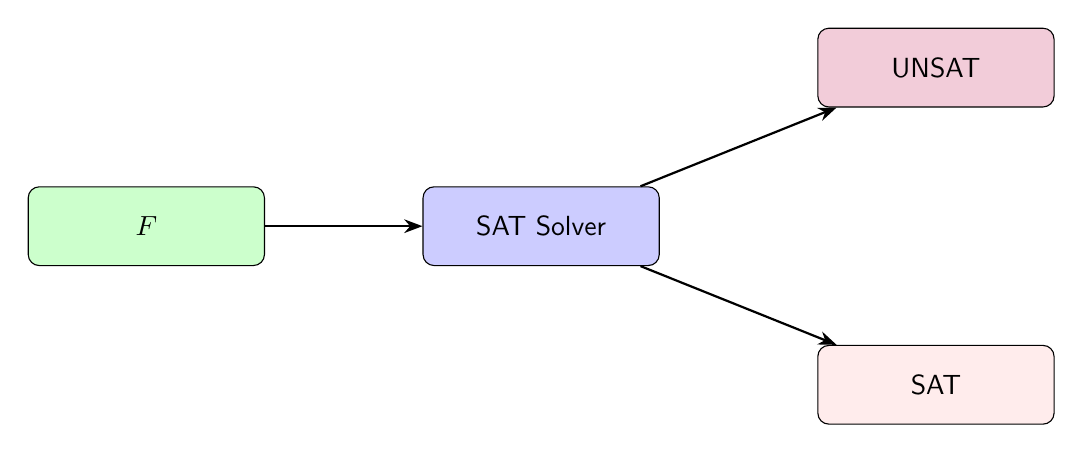
\begin{tikzpicture}[
	node distance=1cm and 2cm,
	process/.style={rectangle, rounded corners, draw, minimum width=3cm, minimum height=1cm, text centered, font=\sffamily},
	arrow/.style={-Stealth, thick},
	pastelgreen/.style={fill=green!20},
	pastelblue/.style={fill=blue!20},
	pastelpink/.style={fill=pink!30},
	pastelpurple/.style={fill=purple!20}
	]
	
	% Nodes
	\node (F) [process, pastelgreen] {$F$};
	\node (SATsolver) [process, pastelblue, right=of F] {SAT Solver};
	\node (SAT) [process, pastelpink, below right=of SATsolver] {SAT};
	\node (UNSAT) [process, pastelpurple, above right=of SATsolver] {UNSAT};
	
	% Arrows
	\draw[arrow] (F) -- (SATsolver);
	\draw[arrow] (SATsolver) -- node[below left] {} (SAT);
	\draw[arrow] (SATsolver) -- node[above left] {} (UNSAT);
\end{tikzpicture}
\end{figure}

\newpage
\subsection{Deciding Validity and Satisfiability}
Two approaches to show $F$ is valid:
\begin{itemize}
	\item \textbf{Truth Table Method} performs exhaustive search: e.g., \[
	F:P\land Q\to P\lor\lnot Q.
	\]
	\begin{table}[h!]\centering
		\begin{tabular}{c|c|c|c|c||c}
			\hline
			$P$ & $Q$ & $P\land Q$ & $\lnot Q$ & $P\lor\lnot Q$ & $F$ \\ \hline
			0 & 0 & 0 & 1 & 1 & 1 \\
			0 & 1 & 0 & 0 & 0 & 1 \\
			1 & 0 & 0 & 1 & 1 & 1 \\
			1 & 1 & 1 & 0 & 1 & 1 \\ \hline
		\end{tabular}
	\end{table} \\
	Non-applicable to logic with infinite domain (e.g., first-order logic).
	\item \textbf{Semantic Argument Method} uses deduction:
	\begin{itemize}
		\item Assume $F$ is valid: $I\not\models F$ for some $I$ (falsifying interpretation).
		\item Apply deduction rules (proof rules) to derive a contradiction.
		\item If every branch of the proof derives a contradiction, then $F$ is valid.
		\item If some branch of the proof never derives a contradiction, then $F$ is invalid.
	\end{itemize}
\end{itemize}

\subsection{Deduction Rules for Propositional Logic}
\begin{center}
\begin{minipage}{.48\textwidth}
	\item \textbf{Negation Elimination}\[
	\frac{I\models\lnot F}{I\not\models F}
	\] This rule shows how to derive $F$ from $\lnot F$. It eliminates the negation by asserting that if $\lnot F$ holds, then $F$ cannot hold.
	\vspace{12pt}
	\item \textbf{Conjunction Elimination}\footnote{And-Elimination}\[
	\frac{I\models F\land G}{I\models F, I\models G}
	\] This rule breaks down a conjunction into its individual components, showing that if 
	$F\land G$ is true, then both $F$ and $G$ are true.
	\vspace{12pt}
	\item \textbf{Disjunction Elimination}\footnote{Or-Elimination} \[
	\frac{I\models F\lor G}{I\models F\mid I\models G}
	\] This rule asserts that if $F\lor G$ is true in an interpretation, then either 
	$F$ is true, or $G$ is true, or both are true. This is also sometimes referred to as the rule of cases.
	\vspace{12pt}
	\item \textbf{Implication Elimination}\footnote{Material Implication}\[
	\frac{I\models F\to G}{I\not\models F\mid I\models G}
	\] This rule states that if $F\to G$ is true in an interpretation, then either 
	$F$ is false or $G$ is true. This corresponds to the definition of material implication in classical logic.
	
	\vspace{12pt}
	\item \textbf{Biconditional Elimination}\footnote{If and Only If Elimination}\[
	\frac{I\models F\leftrightarrow G}{I\models F\land G\mid I\models\lnot F\land\lnot G}
	\] This rule states that if $F\leftrightarrow G$ is true in an interpretation, then either both 
	$F$ and $G$ are true, or both $F$ and $G$ are false. This corresponds to the definition of a biconditional statement in classical logic.
\end{minipage}\quad
\begin{minipage}{.48\textwidth}
\item \textbf{Negation Introduction} \[
\frac{I\not\models \lnot F}{I\models F}
\] This rule introduces $F$ from the fact that $\lnot F$ does not hold. It asserts that if the negation of $F$ does not hold, then $F$ must hold.
\vspace{12pt}
\item \textbf{De Morgan's Law for Conjunction}\footnote{Contrapositive of Conjunction Introduction}\[
\frac{I\not\models F\land G}{I\not\models F \mid I\not\models G}
\] This rule states that if 
$F\land G$ is not true, then at least one of $F$ or $G$ is not true. This is an application of De Morgan's laws.
\vspace{12pt}
\item \textbf{De Morgan's Law for Disjunction}\footnote{Contrapositive of Disjunction Introduction}\[
\frac{I\not\models F\lor G}{I\not\models F, I\not\models G}
\] This rule states that if $F\lor G$ is not true, then both $F$ is not true and $G$ is not true.  This is directly derived from De Morgan's laws in classical logic.
\vspace{12pt}
\item \textbf{Denial of Implication}\footnote{Contrapositive of Implication} \[
\frac{I\not\models F\to G}{I\models F, I\not\models G}
\] This rule states that if $F\to G$ is not true in an interpretation, then 
$F$ must be true and $G$ must be false. This is the contrapositive form of material implication.
\vspace{12pt}
\item \textbf{Negation of Biconditional}\footnote{Exclusive Or Elimination} \[
\frac{I\not\models F\leftrightarrow G}{I\models F\land \lnot G\mid I\models\lnot F\land G}
\] This rule states that if $F\leftrightarrow G$ is not true in an interpretation, then $F$ and 
$G$ have opposite truth values, i.e., either $F$ is true and $G$ is false, or $F$ is false and $G$ is true.
This aligns with the concept of exclusive or (XOR).
\end{minipage}
\end{center}
\begin{center}
\textbf{Contradiction Introduction} (Proof by Contradiction) \[
\frac{I\models F\quad I\not\models F}{I\models\bot}
\]
\end{center}
\begin{example}
	To prove that the formula \[
	F:P\land Q\to P\lor\lnot Q
	\] is valid, assume that it is invalid and derive a contradiction:
	\[
	\begin{array}{ll}
		1.\quad I\not\models P\land \to P\lor\lnot Q & \text{assumption} \\
		2.\quad I\models P\land Q & \text{by 1 and semantics of $\to$} \\
		3.\quad I\not\models P\lor \lnot Q & \text{by 1 and semantics of $\to$} \\
		4.\quad I\models P & \text{by 2 and semantics of $\land$} \\
		5.\quad I\lnot\models P & \text{by 3 and semantics of $\lor$} \\
		6.\quad I\models\bot & \text{4 and 5 are contradictory}
	\end{array}
	\]
\end{example}

\begin{example}
	To prove that the formula \[
	F:(P\to Q)\land(Q\to R)\to(P\to R)
	\] is valid, assume that it is invalid and derive a contradiction:
\end{example}

\subsection{Proof Tree}

A proof evolves as a tree.
\begin{itemize}
	\item A branch is a sequence descending from the root.
	\item A branch is \textit{closed} it contains a contradiction. Otherwise, the branch is \textit{open}.
	\item It is a proof of the validity of $F$ if every branch is closed; otherwise, each open branch describes a falsifying interpretation of $F$.
\end{itemize}

\subsection{Derived Rules}
The proof rules are sufficient, but \textbf{derived rules} can make proofs more concise. E.g., the rule of modus ponens: \[
\frac{I\models F\quad I\models F\to G}{I\models G}
\]
The proof of the validity of the formula:\[
F:(P\to Q)\land (Q\to R)\to (P\to R)
\]
\[
\begin{array}{lll}
	1.& I\not\models F & \text{assumption} \\
	2.& I\models (P\to Q)\land (Q\to R) & \text{by 1 and semantics of $\to$} \\
	3.& I\models P\to R & \text{by 1 and semantics of $\to$} \\
	4.& I\models P & \text{by 3 and semantics of $\to$} \\
	5.& I\not\models R & \text{by 3 and semantics of $\to$} \\
	6.& I\not\models P\to Q & \text{2 and semantics of $\land$} \\
	7.& I\not\models Q\to R & \text{2 and semantics of $\land$} \\
	8.& I\not\models Q & \text{by 4, 6, and modus ponens} \\
	9.& I\not\models R & \text{by 8, 7, and modus ponens} \\
	10.& I\models\bot & \text{5 and 9 are contradictory}
\end{array}
\]


%\subsection*{1. Modus Ponens (MP)}
%\[
%\frac{A, \quad A \rightarrow B}{B}
%\]
%
%\subsection*{2. Modus Tollens (MT)}
%\[
%\frac{A \rightarrow B, \quad \neg B}{\neg A}
%\]
%
%\subsection*{3. Disjunction Introduction (DI)}
%\[
%\frac{A}{A \vee B}
%\]
%\[
%\frac{B}{A \vee B}
%\]
%
%\subsection*{4. Disjunction Elimination (DE)}
%\[
%\frac{A \vee B, \quad \neg A}{B}
%\]
%\[
%\frac{A \vee B, \quad \neg B}{A}
%\]
%
%\subsection*{5. Conjunction Introduction (CI)}
%\[
%\frac{A, \quad B}{A \wedge B}
%\]
%
%\subsection*{6. Conjunction Elimination (CE)}
%\[
%\frac{A \wedge B}{A}
%\]
%\[
%\frac{A \wedge B}{B}
%\]
%
%\subsection*{7. Biconditional Introduction (BI)}
%\[
%\frac{A \rightarrow B, \quad B \rightarrow A}{A \leftrightarrow B}
%\]
%
%\subsection*{8. Biconditional Elimination (BE)}
%\[
%\frac{A \leftrightarrow B}{A \rightarrow B}
%\]
%\[
%\frac{A \leftrightarrow B}{B \rightarrow A}
%\]
%
%\subsection*{9. Negation Introduction (NI)}
%\[
%\frac{A \rightarrow \bot}{\neg A}
%\]
%
%\subsection*{10. Negation Elimination (NE)}
%\[
%\frac{\neg A \rightarrow \bot}{A}
%\]
%
%\subsection*{11. Double Negation Elimination (DNE)}
%\[
%\frac{\neg \neg A}{A}
%\]
%
%\subsection*{12. Contradiction Elimination (CE)}
%\[
%\frac{\bot}{A}
%\]
%
%\subsection*{13. Contradiction Introduction (CI)}
%\[
%\frac{A \wedge \neg A}{\bot}
%\]
	
	\newpage
	\chapter{Propositional Logic I}
	% Propositional Logic I

References:\cite{youtube:COSE419-Lecture4-1}

Propositional logic is a branch of logic that deals with propositions which can be either true or false. The basic components and operations in propositional logic are as follows:

%\begin{align*}
%	\texttt{<atom>} ::= &\ \text{"P"}\ |\ \text{"Q"}\ |\ \text{"R"}\ |\ \ldots\
%\end{align*}
%
%\begin{align*}
%	\texttt{<literal>} ::= &\ \texttt{<atom>} \\
%	&\ |\ \text{"¬"}\ \texttt{<atom>}
%\end{align*}
%
%\begin{align*}
%	\texttt{<formula>} ::= &\ \texttt{<literal>} \\
%	&\ |\ \text{"("}\ \texttt{<formula>}\ \text{")"} \\
%	&\ |\ \text{"¬"}\ \texttt{<formula>} \\
%	&\ |\ \text{"("}\ \texttt{<formula>}\ \text{"∧"}\ \texttt{<formula>}\ \text{")"} \\
%	&\ |\ \text{"("}\ \texttt{<formula>}\ \text{"∨"}\ \texttt{<formula>}\ \text{")"} \\
%	&\ |\ \text{"("}\ \texttt{<formula>}\ \text{"→"}\ \texttt{<formula>}\ \text{")"} \\
%	&\ |\ \text{"("}\ \texttt{<formula>}\ \text{"↔"}\ \texttt{<formula>}\ \text{")"} \\
%\end{align*}

\section{Syntax and Semantic of Propositional Logic}
\begin{center}
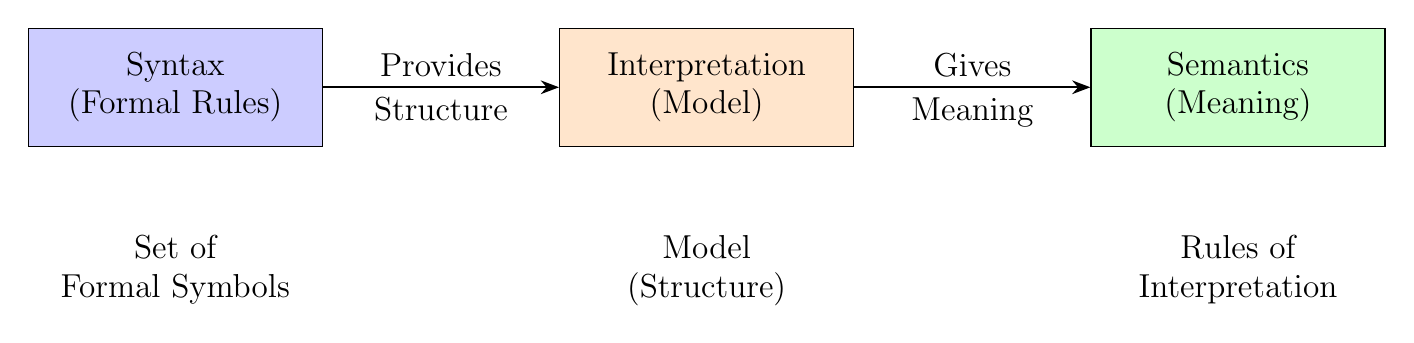
\begin{tikzpicture}[
	every node/.style={font=\large, node distance=3cm},
	process/.style={rectangle, draw, text width=3.5cm, align=center, minimum height=1.5cm},
	arrow/.style={thick, ->, >=Stealth}
	]
	
	% Nodes
	\node[process, fill=blue!20] (syntax) {Syntax \\ (Formal Rules)};
	\node[process, fill=orange!20, right=of syntax] (interpretation) {Interpretation \\ (Model)};
	\node[process, fill=green!20, right=of interpretation] (semantics) {Semantics \\ (Meaning)};
	
	% Arrows
	\draw[arrow] (syntax) -- node[above, align=center] {Provides} node[below, align=center] {Structure} (interpretation);
	\draw[arrow] (interpretation) -- node[above, align=center] {Gives} node[below, align=center] {Meaning} (semantics);
	
	% Labels
	\node[below=1cm of syntax, align=center] {Set of \\ Formal Symbols};
	\node[below=1cm of interpretation, align=center] {Model \\ (Structure)};
	\node[below=1cm of semantics, align=center] {Rules of \\ Interpretation};
\end{tikzpicture}
\end{center}
\subsection{Syntax}
% Tree illustrating Atoms, Literals, and Formulas
\begin{center}\adjustbox{scale=.75}{
%\begin{tikzpicture}[
%	level distance=2.5cm,
%	sibling distance=3.5cm,
%	every node/.style={draw, shape=rectangle, rounded corners, align=center}
%	]
%	
%	% Root
%	\node {Boolean Logic}
%	% Level 1
%	child {node {Unary}
%	}
%	child {node {Binary}
%	}
%	% Level 2
%	child {node {Atom}
%		% Level 3 for Unary
%		child {node {Unary: $\bot$ (false)}}
%		child {node {Unary: $\top$ (true)}}
%		% Level 3 for Binary
%		child {node {Binary: $P, Q, R, \dots$}}
%	}
%	child {node {Literal}
%		% Level 3 for Unary
%		child {node {Unary: $\neg \bot$}}
%		child {node {Unary: $\neg \top$}}
%		% Level 3 for Binary
%		child {node {Binary: $\neg P, \neg Q, \neg R, \dots$}}
%	}
%	child {node {Formula}
%		% Level 3 for Unary
%		child {node {Unary: $\neg F$ (not)}}
%		% Level 3 for Binary
%		child {node {Binary: $F_1 \land F_2$ (and)}}
%		child {node {Binary: $F_1 \lor F_2$ (or)}}
%		child {node {Binary: $F_1 \to F_2$ (implies)}}
%		child {node {Binary: $F_1 \leftrightarrow F_2$ (if and only if)}}
%	};
%	
%\end{tikzpicture}
}
\end{center}
%\begin{tikzpicture}[
%	node distance=2cm,
%	every node/.style={draw, rectangle, rounded corners, align=center},
%	level 1/.style={sibling distance=6cm},
%	level 2/.style={sibling distance=3cm},
%	level 3/.style={sibling distance=2cm}
%	]
%	
%	% Root node
%	\node (formula) {Formula};
%	
%	% Level 1
%	\node [below left=of formula] (literal) {Literal}
%	child {node (atom) {Atom\\(e.g., $P, Q$)}}
%	child {node (negatom) {Negation of Atom\\(e.g., $\lnot P, \lnot Q$)}};
%	
%	\node [below right=of formula] (special) {Special Constant}
%	child {node {True\\($\top$)}}
%	child {node {False\\($\bot$)}};
%	
%	% Connections from Formula to Literals and Special Constants
%	\draw (formula) -- (literal);
%	\draw (formula) -- (special);
%	
%	% Level 2
%	\node [below=2cm of literal] (unary) {Unary Truth Function}
%	child {node (neg) {Negation\\($\lnot F$)}};
%	
%	\node [below=2cm of special] (binary) {Binary Truth Function}
%	child {node (and) {Conjunction\\($F_1 \land F_2$)}}
%	child {node (or) {Disjunction\\($F_1 \lor F_2$)}}
%	child {node (imp) {Implication\\($F_1 \to F_2$)}}
%	child {node (bicond) {Biconditional\\($F_1 \leftrightarrow F_2$)}};
%	
%	% Connections from Literals to Unary Truth Function
%	\draw (literal) -- (unary);
%	
%	% Connections from Special Constants to Binary Truth Function
%	\draw (special) -- (binary);
%	
%	% Level 3 Connections from Unary and Binary Truth Functions to Formulas
%	\foreach \child in {neg, and, or, imp, bicond}
%	\draw (\child) -- ++(0,-1) node[draw, rectangle, rounded corners, align=center] {Formula};
%	
%	% Additional connections to demonstrate usage
%	\draw (negatom) -- (neg);
%	\draw (atom) -- (unary);
%	\draw (negatom) -- (unary);
%	
%\end{tikzpicture}
\begin{itemize}
	\item \textbf{Atom}: basic elements
	\begin{itemize}
		\item truth symbols $\bot$(``false'') and $\top$(``true'')
		\item propositional variables $P,Q,R,\dots$
	\end{itemize}
	\item \textbf{Literal}: an atom $\alpha$ or its negation $\lnot\alpha$.
	\item \textbf{Formula}: a literal or the application of a logical connective (boolean connectives) to formulas
	\[
	\begin{array}{ccll}
		F & \to & \bot \\
		& | & \top \\
		& | & P \\
		& | & \lnot F & \text{negation (``not'')} \\
		& | & F_1\land F_2 & \text{conjunction (``and'')} \\
		& | & F_1\lor F_2 & \text{disjunction (``or'')} \\
		& | & F_1\to F_2 & \text{implication (``implies'')} \\
		& | & F_1\leftrightarrow F_2 & \text{iff (``if and only if'')}
	\end{array}
	\]
	\item[]
	\item Formula $G$ is a \textbf{subformula} of formula $F$ if it occurs syntactically within $G$.
	\begin{align*}
		\sub{\bot} &= \set{\bot} \\
		\sub{\top} &= \set{\top} \\
		\sub{P} &= \set{P} \\
		\sub{\lnot F} &= \set{\lnot F}\cup\sub{F} \\
		\sub{F_1\land F_2} &= \set{F_1\land F_2}\cup\sub{F_1}\cup\sub{F_2}
		&\vdots
	\end{align*}
	\item Consider $F:(P\land Q)\to (P\lor\lnot Q)$. Then \[
	\sub{F}=\set{F,P\land Q,P\lor\lnot Q,P,Q,\lnot Q}.
	\]
	\begin{center}\begin{minipage}{.45\textwidth}\centering\adjustbox{scale=.8}{
%\begin{tikzpicture}[
%%	sibling distance=8cm,
%%	level distance=2cm,
%	every node/.style = {shape=rectangle, rounded corners, draw, align=center},
%	level 1/.style = {sibling distance=2cm, level distance=1cm},
%	level 2/.style = {sibling distance=1cm, level distance=1cm},
%	level 3/.style = {sibling distance=1cm, level distance=1cm}
%%	edge from parent/.style = {draw, -{Latex}, thick},
%%	edge from parent path = {(\tikzparentnode.south) -- ++(0,-1.5em) -| (\tikzchildnode.north)}
%	]
%	\node {$(P\land Q)\to(P\lor\lnot Q)$}
%	child { node {$P\land Q$}
%		child { node {$P$} }
%		child { node {$Q$} }
%	}
%	child { node {$P\lor\lnot Q$}
%		child { node {$P$}
%		}
%		child { node {$\lnot Q$} 
%			child { node {$Q$} } 
%		}
%	};
%\end{tikzpicture}
\begin{tikzcd}
	& (P\land Q)\to(P\lor\lnot Q) \arrow[ld, no head] \arrow[rd, no head] &                                                      \\
	P\land Q \arrow[dd, no head] \arrow[rdd, no head] &                                                                     & P\lor\lnot Q \arrow[d, no head] \arrow[ldd, no head] \\
	&                                                                     & \lnot Q                                              \\
	Q                                                 & P                                                                   &          
\end{tikzcd}
}
\end{minipage}
\begin{minipage}{.45\textwidth}\centering\adjustbox{scale=.8}{
\begin{tikzcd}
	P \arrow[ddd, no head] \arrow[rrddd, no head] &                          & Q \arrow[d, no head] \arrow[llddd, no head] \\
	&                          & \lnot Q \arrow[dd, no head]                 \\
	&                          &                                             \\
	P\land Q \arrow[rdd, no head]                 &                          & P\lor\lnot Q \arrow[ldd, no head]           \\
	&                          &                                             \\
	& P\land Q\to P\lor\lnot Q &                                            
\end{tikzcd}}
\end{minipage}	
%\begin{minipage}{.48\textwidth}\adjustbox{scale=.5}{
%		\begin{tikzpicture}[
%			edge from parent/.style={draw, -latex},
%			sibling distance=4cm,
%			level distance=2cm,
%			every node/.style={draw, shape=rectangle, rounded corners, align=center}
%			]
%			
%			% Unary and Binary Nodes
%			\node {Boolean Logic}
%			child {node {Unary}
%				child {node {Atom}}
%				child {node {Literal}}
%				child {node {Formula}}
%			}
%			child {node {Binary}
%				child {node {Atom}}
%				child {node {Literal}}
%				child {node {Formula}}
%			};
%			
%			% Atom, Literal, and Formula Nodes
%			\node (atom) [below=4cm of Boolean-1-1] {Atom}
%			child {node {$\bot$}}
%			child {node {$\top$}};
%			\node (literal) [below=4cm of Boolean-1-2] {Literal}
%			child {node {$\neg \alpha$}};
%			\node (formula) [below=4cm of Boolean-1-3] {Formula}
%			child {node {$F$}}
%			child {node {$\neg F$}};
%			
%			% Connections to common nodes
%			\draw[-] (Boolean-1-1) -- (atom);
%			\draw[-] (Boolean-2-1) -- (atom);
%			\draw[-] (Boolean-1-2) -- (literal);
%			\draw[-] (Boolean-2-2) -- (literal);
%			\draw[-] (Boolean-1-3) -- (formula);
%			\draw[-] (Boolean-2-3) -- (formula);
%	\end{tikzpicture}
%\end{minipage}
\end{center}
	\item The strict subformulas of a formula are all its subformulas except itself.
	\item[]
	\item To minimally use parentheses, we define the relative precedence of the logical connectives from highest to lowest as follows: \[
	\lnot\quad\land\quad\lor\quad\rightarrow\quad\leftrightarrow
	\]
	\item (Currying) Additionally, $\rightarrow$ and $\leftrightarrow$ associate to the right, e.g., \[
	P\to Q\to R\iff P\to(Q\to R).
	\]
	\item Example:
	\begin{itemize}
		\item $(P\land Q)\to (P\lor\lnot Q)\iff P\land Q\to P\lor \lnot Q$
		\item $(P_1\land((\lnot P_2)\land\top))\lor((\lnot P_1)\land P_2)\iff P_1\land P_2\top\lor\lnot P_1\land P_2$
	\end{itemize}
\end{itemize}

\subsection{Semantics}
\begin{itemize}
	\item The semantics of a logic provides its meaning. The meaning of a PL formula is either true or false.
	\item The semantics of a formula is defined with an \textbf{interpretation} (or assignment) that assigns truth values to propositional variables.
	\item For example, $F:P\land Q\to P\lor\land Q$ evaluates to true under the interpretation $I:\set{P\mapsto \text{true},Q\mapsto\text{false}}:$
	\begin{table}[h!]\centering\setstretch{1.25}
		\begin{tabular}{c|c||c|c|c|c}
			\hline
			$P$ & $Q$ & $\lnot Q$ & $P\land Q$ & $P\lor \lnot Q$ & $F$ \\ \hline
			1 & 0 & 1 & 0 & 1 & 1 \\ \hline
		\end{tabular}
	\end{table}
	\item The tabular notation is unsuitable for predicate logic. Instead, we define the semantics inductively.
\end{itemize}

\subsection{Inductive Definition of Semantics}
In an inductive definition, the meaning of basic elements is defined first.
The meaning of complex elements is defined in terms of subcomponents.
\begin{itemize}
	\item We write $I\models F$ if $F$ evaluates to \textbf{true} under $I$.
	\item We write $I\not\models F$ if $F$ evaluates to \textbf{false} under $I$.
\end{itemize}
Note that \[
\begin{array}{ll}
I\models \top,\quad I\not\models\bot, & \\
I\models P &\text{iff}\ I[P]=\text{true} \\
I\models \lnot F &\text{iff}\ I[P]=\text{false} \\
I\models\lnot F &\text{iff}\ I\not\models F \\
I\models F_1\land F_2 &\text{iff}\ I\models F_1\ \text{and}\ I\models F_2 \\
I\models F_1\lor F_2 &\text{iff}\ I\models F_1\ \text{or}\ I\models F_2 \\
I\models F_1\to F_2 &\text{iff}\ I\not\models F_1\ \text{or}\ I\models F_2 \\
I\models F_1\leftrightarrow F_2 &\text{iff}\ (I\models F_1\ \text{and}\ I\models F_2)\ \text{or}\ (I\not\models F_1\ \text{and}\ I\not\models F_2)
\end{array}
\]
\vspace{12pt}
\begin{example}
	Consider the formula \[
	F:P\land Q\to P\lor\lnot Q
	\] and the interpretation \[
	I:\set{P\mapsto\text{true},Q\mapsto\text{false}}.
	\] The truth value of $F$ is computed as follows: \[
	\begin{array}{ll}
		1.\quad I\models P &\text{since $I[P]=\text{true}$} \\
		2.\quad I\not\models Q &\text{since $I[P]=\text{true}$} \\
		3.\quad I\models \lnot Q &\text{by 2 and semantics of $\lnot$} \\
		4.\quad I\not\models P\land Q &\text{by 2 and semantics of $\land$} \\
		5.\quad I\models P\lor \lnot Q &\text{by 1 and semantics of $\lor$} \\
		6.\quad I\models F &\text{by 4 and semantics of $\to$} \\
	\end{array}
	\]
\end{example}

\section{Satisfiability and Validity}
\begin{itemize}
	\item A formula $F$ is \textbf{satisfiable} iff there exists an interpretation $I$ such that $I\models F$.
	\item A formula $F$ is \textbf{valid} iff for all interpretations $I$, $I\models F$.
	\item Satisfiability and validity are dual: \[
	\text{$F$ is valid}\iff\text{$\lnot F$ is unsatisfiable}
	\]
	\begin{proof}
		content...
	\end{proof}
	\item We can check satisfiability by deciding validity, and vice versa.
\end{itemize}

\begin{figure}[h!]\centering
\begin{tikzcd}
	& \text{VALID} \arrow[dr, "\neg"] & \\
	\text{SAT} \arrow[ur, "\neg"] \arrow[rr, "\neg"] & & \text{UNSAT} \\
	& \text{INVALID} \arrow[ul, "\neg"] \arrow[ur, "\neg"] &
\end{tikzcd}
\caption{Relation of SAT, UNSAT, VALID and INVALID}
\end{figure}

\begin{figure}[h!]\centering
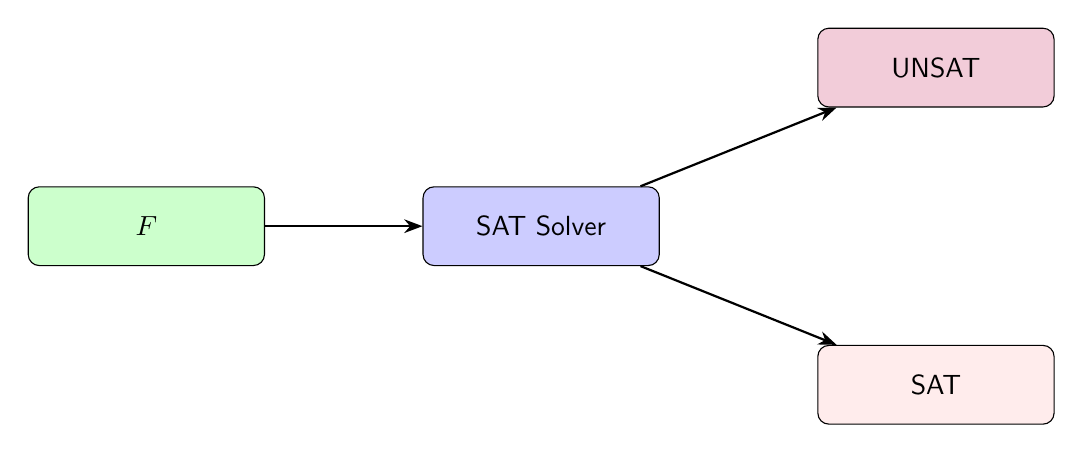
\begin{tikzpicture}[
	node distance=1cm and 2cm,
	process/.style={rectangle, rounded corners, draw, minimum width=3cm, minimum height=1cm, text centered, font=\sffamily},
	arrow/.style={-Stealth, thick},
	pastelgreen/.style={fill=green!20},
	pastelblue/.style={fill=blue!20},
	pastelpink/.style={fill=pink!30},
	pastelpurple/.style={fill=purple!20}
	]
	
	% Nodes
	\node (F) [process, pastelgreen] {$F$};
	\node (SATsolver) [process, pastelblue, right=of F] {SAT Solver};
	\node (SAT) [process, pastelpink, below right=of SATsolver] {SAT};
	\node (UNSAT) [process, pastelpurple, above right=of SATsolver] {UNSAT};
	
	% Arrows
	\draw[arrow] (F) -- (SATsolver);
	\draw[arrow] (SATsolver) -- node[below left] {} (SAT);
	\draw[arrow] (SATsolver) -- node[above left] {} (UNSAT);
\end{tikzpicture}
\end{figure}

\newpage
\subsection{Deciding Validity and Satisfiability}
Two approaches to show $F$ is valid:
\begin{itemize}
	\item \textbf{Truth Table Method} performs exhaustive search: e.g., \[
	F:P\land Q\to P\lor\lnot Q.
	\]
	\begin{table}[h!]\centering
		\begin{tabular}{c|c|c|c|c||c}
			\hline
			$P$ & $Q$ & $P\land Q$ & $\lnot Q$ & $P\lor\lnot Q$ & $F$ \\ \hline
			0 & 0 & 0 & 1 & 1 & 1 \\
			0 & 1 & 0 & 0 & 0 & 1 \\
			1 & 0 & 0 & 1 & 1 & 1 \\
			1 & 1 & 1 & 0 & 1 & 1 \\ \hline
		\end{tabular}
	\end{table} \\
	Non-applicable to logic with infinite domain (e.g., first-order logic).
	\item \textbf{Semantic Argument Method} uses deduction:
	\begin{itemize}
		\item Assume $F$ is valid: $I\not\models F$ for some $I$ (falsifying interpretation).
		\item Apply deduction rules (proof rules) to derive a contradiction.
		\item If every branch of the proof derives a contradiction, then $F$ is valid.
		\item If some branch of the proof never derives a contradiction, then $F$ is invalid.
	\end{itemize}
\end{itemize}

\subsection{Deduction Rules for Propositional Logic}
\begin{center}
\begin{minipage}{.48\textwidth}
	\item \textbf{Negation Elimination}\[
	\frac{I\models\lnot F}{I\not\models F}
	\] This rule shows how to derive $F$ from $\lnot F$. It eliminates the negation by asserting that if $\lnot F$ holds, then $F$ cannot hold.
	\vspace{12pt}
	\item \textbf{Conjunction Elimination}\footnote{And-Elimination}\[
	\frac{I\models F\land G}{I\models F, I\models G}
	\] This rule breaks down a conjunction into its individual components, showing that if 
	$F\land G$ is true, then both $F$ and $G$ are true.
	\vspace{12pt}
	\item \textbf{Disjunction Elimination}\footnote{Or-Elimination} \[
	\frac{I\models F\lor G}{I\models F\mid I\models G}
	\] This rule asserts that if $F\lor G$ is true in an interpretation, then either 
	$F$ is true, or $G$ is true, or both are true. This is also sometimes referred to as the rule of cases.
	\vspace{12pt}
	\item \textbf{Implication Elimination}\footnote{Material Implication}\[
	\frac{I\models F\to G}{I\not\models F\mid I\models G}
	\] This rule states that if $F\to G$ is true in an interpretation, then either 
	$F$ is false or $G$ is true. This corresponds to the definition of material implication in classical logic.
	
	\vspace{12pt}
	\item \textbf{Biconditional Elimination}\footnote{If and Only If Elimination}\[
	\frac{I\models F\leftrightarrow G}{I\models F\land G\mid I\models\lnot F\land\lnot G}
	\] This rule states that if $F\leftrightarrow G$ is true in an interpretation, then either both 
	$F$ and $G$ are true, or both $F$ and $G$ are false. This corresponds to the definition of a biconditional statement in classical logic.
\end{minipage}\quad
\begin{minipage}{.48\textwidth}
\item \textbf{Negation Introduction} \[
\frac{I\not\models \lnot F}{I\models F}
\] This rule introduces $F$ from the fact that $\lnot F$ does not hold. It asserts that if the negation of $F$ does not hold, then $F$ must hold.
\vspace{12pt}
\item \textbf{De Morgan's Law for Conjunction}\footnote{Contrapositive of Conjunction Introduction}\[
\frac{I\not\models F\land G}{I\not\models F \mid I\not\models G}
\] This rule states that if 
$F\land G$ is not true, then at least one of $F$ or $G$ is not true. This is an application of De Morgan's laws.
\vspace{12pt}
\item \textbf{De Morgan's Law for Disjunction}\footnote{Contrapositive of Disjunction Introduction}\[
\frac{I\not\models F\lor G}{I\not\models F, I\not\models G}
\] This rule states that if $F\lor G$ is not true, then both $F$ is not true and $G$ is not true.  This is directly derived from De Morgan's laws in classical logic.
\vspace{12pt}
\item \textbf{Denial of Implication}\footnote{Contrapositive of Implication} \[
\frac{I\not\models F\to G}{I\models F, I\not\models G}
\] This rule states that if $F\to G$ is not true in an interpretation, then 
$F$ must be true and $G$ must be false. This is the contrapositive form of material implication.
\vspace{12pt}
\item \textbf{Negation of Biconditional}\footnote{Exclusive Or Elimination} \[
\frac{I\not\models F\leftrightarrow G}{I\models F\land \lnot G\mid I\models\lnot F\land G}
\] This rule states that if $F\leftrightarrow G$ is not true in an interpretation, then $F$ and 
$G$ have opposite truth values, i.e., either $F$ is true and $G$ is false, or $F$ is false and $G$ is true.
This aligns with the concept of exclusive or (XOR).
\end{minipage}
\end{center}
\begin{center}
\textbf{Contradiction Introduction} (Proof by Contradiction) \[
\frac{I\models F\quad I\not\models F}{I\models\bot}
\]
\end{center}
\begin{example}
	To prove that the formula \[
	F:P\land Q\to P\lor\lnot Q
	\] is valid, assume that it is invalid and derive a contradiction:
	\[
	\begin{array}{ll}
		1.\quad I\not\models P\land \to P\lor\lnot Q & \text{assumption} \\
		2.\quad I\models P\land Q & \text{by 1 and semantics of $\to$} \\
		3.\quad I\not\models P\lor \lnot Q & \text{by 1 and semantics of $\to$} \\
		4.\quad I\models P & \text{by 2 and semantics of $\land$} \\
		5.\quad I\lnot\models P & \text{by 3 and semantics of $\lor$} \\
		6.\quad I\models\bot & \text{4 and 5 are contradictory}
	\end{array}
	\]
\end{example}

\begin{example}
	To prove that the formula \[
	F:(P\to Q)\land(Q\to R)\to(P\to R)
	\] is valid, assume that it is invalid and derive a contradiction:
\end{example}

\subsection{Proof Tree}

A proof evolves as a tree.
\begin{itemize}
	\item A branch is a sequence descending from the root.
	\item A branch is \textit{closed} it contains a contradiction. Otherwise, the branch is \textit{open}.
	\item It is a proof of the validity of $F$ if every branch is closed; otherwise, each open branch describes a falsifying interpretation of $F$.
\end{itemize}

\subsection{Derived Rules}
The proof rules are sufficient, but \textbf{derived rules} can make proofs more concise. E.g., the rule of modus ponens: \[
\frac{I\models F\quad I\models F\to G}{I\models G}
\]
The proof of the validity of the formula:\[
F:(P\to Q)\land (Q\to R)\to (P\to R)
\]
\[
\begin{array}{lll}
	1.& I\not\models F & \text{assumption} \\
	2.& I\models (P\to Q)\land (Q\to R) & \text{by 1 and semantics of $\to$} \\
	3.& I\models P\to R & \text{by 1 and semantics of $\to$} \\
	4.& I\models P & \text{by 3 and semantics of $\to$} \\
	5.& I\not\models R & \text{by 3 and semantics of $\to$} \\
	6.& I\not\models P\to Q & \text{2 and semantics of $\land$} \\
	7.& I\not\models Q\to R & \text{2 and semantics of $\land$} \\
	8.& I\not\models Q & \text{by 4, 6, and modus ponens} \\
	9.& I\not\models R & \text{by 8, 7, and modus ponens} \\
	10.& I\models\bot & \text{5 and 9 are contradictory}
\end{array}
\]


%\subsection*{1. Modus Ponens (MP)}
%\[
%\frac{A, \quad A \rightarrow B}{B}
%\]
%
%\subsection*{2. Modus Tollens (MT)}
%\[
%\frac{A \rightarrow B, \quad \neg B}{\neg A}
%\]
%
%\subsection*{3. Disjunction Introduction (DI)}
%\[
%\frac{A}{A \vee B}
%\]
%\[
%\frac{B}{A \vee B}
%\]
%
%\subsection*{4. Disjunction Elimination (DE)}
%\[
%\frac{A \vee B, \quad \neg A}{B}
%\]
%\[
%\frac{A \vee B, \quad \neg B}{A}
%\]
%
%\subsection*{5. Conjunction Introduction (CI)}
%\[
%\frac{A, \quad B}{A \wedge B}
%\]
%
%\subsection*{6. Conjunction Elimination (CE)}
%\[
%\frac{A \wedge B}{A}
%\]
%\[
%\frac{A \wedge B}{B}
%\]
%
%\subsection*{7. Biconditional Introduction (BI)}
%\[
%\frac{A \rightarrow B, \quad B \rightarrow A}{A \leftrightarrow B}
%\]
%
%\subsection*{8. Biconditional Elimination (BE)}
%\[
%\frac{A \leftrightarrow B}{A \rightarrow B}
%\]
%\[
%\frac{A \leftrightarrow B}{B \rightarrow A}
%\]
%
%\subsection*{9. Negation Introduction (NI)}
%\[
%\frac{A \rightarrow \bot}{\neg A}
%\]
%
%\subsection*{10. Negation Elimination (NE)}
%\[
%\frac{\neg A \rightarrow \bot}{A}
%\]
%
%\subsection*{11. Double Negation Elimination (DNE)}
%\[
%\frac{\neg \neg A}{A}
%\]
%
%\subsection*{12. Contradiction Elimination (CE)}
%\[
%\frac{\bot}{A}
%\]
%
%\subsection*{13. Contradiction Introduction (CI)}
%\[
%\frac{A \wedge \neg A}{\bot}
%\]
	
	\newpage
	\chapter{Propositional Logic II}
	% Propositional Logic II

\cite{youtube:COSE419-Lecture4-1}
\cite{youtube:COSE419-Lecture4-2}
\cite{youtube:COSE419-Lecture4-3}

\section{Equivalence and Implication, and Equisatisfiability}

\subsection{Equivalence and Implication}
\begin{itemize}
	\item Two formulas $F_1$ and $F_2$ are equivalent \[
		F_1\iff F_2
	\] iff $F_1\leftrightarrow F_2$ is valid, \ie, for all interpretations $I$, $I\models F_1\leftrightarrow F_2$.
	\item Formula $F_1$ implies formula $F_2$ \[
	F_1\implies F_2
	\] iff $F_1\to F_2$ is valid, \ie, for all interpretations $I$, $I\models F_1\to F_2$.
	\item $F_1\iff F_2$ and $F_1\implies F_2$ are not formulas. They are semantic assertions.
	\item We can check equivalence and implication by checking satisfiability.
\end{itemize}
\begin{example}
\ \begin{itemize}
	\item $P\iff\lnot\lnot P$ means that $P\leftrightarrow \lnot\lnot p$ is valid.
	\item $P\to Q\iff \lnot P\lor Q$ means that $P\to Q\leftrightarrow \lnot P\lor Q$ is valid.
\end{itemize}
\end{example}
\begin{exercise}
	Prove that \[
	R\land(\lnot R\lor P)\implies P.
	\]
	\begin{proof}[\sol]
		We want to show that $R\land(\lnot R\lor P)\to P$ is valid.
		\[\begin{array}{lll}
			1. & I\models R\land(\lnot R\lor P) & \\
			2. & I\not\models P & \\
			3. & I\models R & \\
			4. & 
		\end{array}
		\]
	\end{proof}
\end{exercise}

\section{Substitution}
\begin{center}
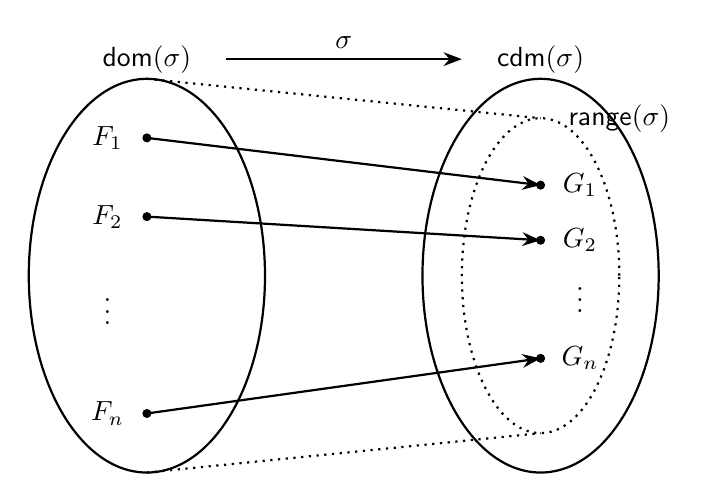
\begin{tikzpicture}
	% Draw the sets A and B
	\draw[thick] (-2.5,0) ellipse (1.5 and 2.5);
	\draw[thick] (2.5,0) ellipse (1.5 and 2.5);
	\draw[dotted, thick] (2.5,0) ellipse (1 and 2);
	
	% Labels for sets
	\node at (-2.5, 2.75) {$\dom(\sigma)$};
	\node at (2.5, 2.75) {$\cdm(\sigma)$};
	\node at (3.5, 2) {$\range(\sigma)$};
	
	% Draw the arrows representing the function
	\draw[-Stealth, thick] (-1.5, 2.75) -- (1.5,2.75) node[midway, above] {$\sigma$};
	\draw[dotted, thick] (-2.5, 2.5) -- (2.5,2);
	\draw[dotted, thick] (-2.5, -2.5) -- (2.5,-2);
	
	\node at (-3, 1.75) {$F_1$};
	\node at (-3, .75) {$F_2$};
	\node at (-3, -.35) {$\vdots$};
	\node at (-3, -1.75) {$F_n$};
	\draw[fill] (-2.5,1.75) circle (.05);
	\draw[fill] (-2.5, .75) circle (.05);
	\draw[fill] (-2.5, -1.75) circle (.05);
	
	\node at (3, 1.15) {$G_1$};
	\node at (3, .45) {$G_2$};
	\node at (3, -.2) {$\vdots$};
	\node at (3, -1.05) {$G_n$};
	\draw[fill] (2.5,1.15) circle (.05);
	\draw[fill] (2.5,.45) circle (.05);
	\draw[fill] (2.5,-1.05) circle (.05);
	
	\draw[-Stealth, thick] (-2.5, 1.75) -- (2.5, 1.15);
	\draw[-Stealth, thick] (-2.5, .75) -- (2.5, .45);
	\draw[-Stealth, thick] (-2.5, -1.75) -- (2.5, -1.05);
\end{tikzpicture}
\end{center}
\subsection{Substitution}
\begin{itemize}
	\item A substitution $\sigma$ is a mapping from formulas to formulas: \[
	\sigma:\set{F_1\mapsto G_1,\dots, F_n\mapsto G_n}
	\]
	\item The domain of $\sigma, \dom(\sigma)$, is \[
	\dom(\sigma)=\set{F_1,\dots,F_n}
	\] while the range is $\range(\sigma)$ \[
	\range(\sigma):\set{G_1,\dots,G_n}.
	\]
	\item The application of a substitution $\sigma$ to a formula $F$, $F\sigma$, replaces each occurence of $F_i$ with $G_i$. Replacements occur all at once.
	\item When two subformulas $F_j$ and $F_k$ are in $\dom(\sigma)$ and $F_k$ strict subformula of $F_j$, then $F_j$ is replaced first.
\end{itemize}

\begin{example}
Consider formula \[
F:P\land Q\to P\lor\lnot Q
\] and substitution \[
\sigma:\set{P\mapsto R,P\land Q\mapsto P\to Q}.
\] Then \[
F\sigma:(P\to Q)\to R\lor\lnot Q.
\] Note that $F\sigma\neq(R\to Q)\to R\lor\lnot Q$.
\begin{center}
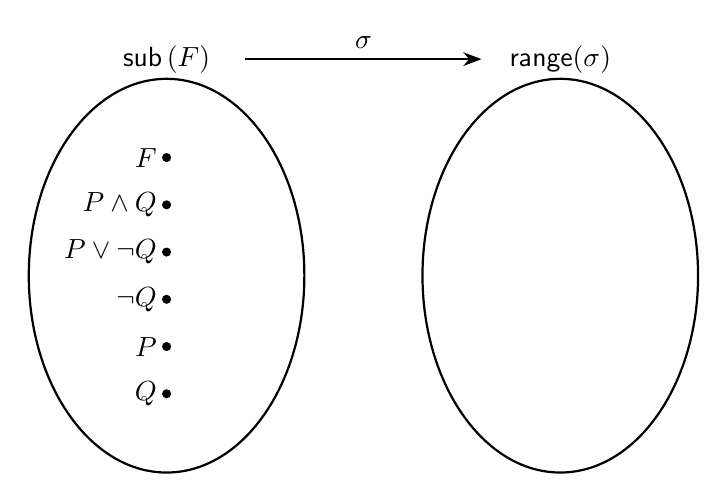
\begin{tikzpicture}
	% Draw the sets A and B
	\draw[thick] (-2.5,0) ellipse (1.75 and 2.5);
	\draw[thick] (2.5,0) ellipse (1.75 and 2.5);
%	\draw[dotted, thick] (2.5,0) ellipse (1 and 2);
	
	% Labels for sets
	\node at (-2.5, 2.75) {$\sub{F}$};
	\node at (2.5, 2.75) {$\range(\sigma)$};
	
	% Draw the arrows representing the function
	\draw[-Stealth, thick] (-1.5, 2.75) -- (1.5,2.75) node[midway, above] {$\sigma$};
%	\draw[dotted, thick] (-2.5, 2.5) -- (2.5,2);
%	\draw[dotted, thick] (-2.5, -2.5) -- (2.5,-2);
	
%	\node at (-3, 1.75) {$F$};
%	\node at (-3, .75) {$P\land Q$};
%	\node at (-3, -.35) {$P\lor\lnot Q$};
%	\node at (-3, -1.75) {$F_n$};
	\draw[fill] (-2.5,1.5) circle (.05) node[left] {$F$};
	\draw[fill] (-2.5, .9) circle (.05) node[left] {$P\land Q$};
	\draw[fill] (-2.5, .3) circle (.05) node[left] {$P\lor\lnot Q$};
	\draw[fill] (-2.5, -.3) circle (.05) node[left] {$\lnot Q$};
	\draw[fill] (-2.5, -.9) circle (.05) node[left] {$P$};
	\draw[fill] (-2.5, -1.5) circle (.05) node[left] {$Q$};
%	
%	\node at (3, 1.15) {$G_1$};
%	\node at (3, .45) {$G_2$};
%	\node at (3, -.2) {$\vdots$};
%	\node at (3, -1.05) {$G_n$};
%	\draw[fill] (2.5,1.15) circle (.05);
%	\draw[fill] (2.5,.45) circle (.05);
%	\draw[fill] (2.5,-1.05) circle (.05);
%	
%	\draw[-Stealth, thick] (-2.5, 1.75) -- (2.5, 1.15);
%	\draw[-Stealth, thick] (-2.5, .75) -- (2.5, .45);
%	\draw[-Stealth, thick] (-2.5, -1.75) -- (2.5, -1.05);
\end{tikzpicture}
\end{center}
\end{example}

\begin{itemize}
	\item A variable substitution is a substitution in which the domain consists only of propositional variables.
	\item When we write $F[F_1,\dots,F_n]$, we mean that formula $F$ and have formulas $F_1,\dots,F_n$ as subformulas.
	\item \[
	\sigma:\set{F_1\mapsto G_1,\dots,F_n\mapsto G_n}\implies F[F_1,\dots,F_n]\sigma:F[G_1,\dots, G_n].
	\]
	\item For example, in the previous example, writing \[
	F[P,P\land Q]\sigma:F[R,P\to Q]
	\] emphasizes that $P$ and $P\land Q$ are replaced by $R$ and $P\to Q$, respectively.
\end{itemize}

\subsection{Semantic Consequences of Substitution}

\lembox[Substitution of Equivalent Formulas]{\begin{lemma}
Consider substitution $\sigma:\set{F_1\mapsto G_1,\dots,F_n\mapsto G_n}$ such that for each $i$, $F_i\iff G_i$. Then, \[
F\iff F\sigma
\]
\end{lemma}}
\begin{example}
	Applying $\sigma:\set{F_1\mapsto G_1,\dots,F_n\mapsto G_n}$ to $F:(P\to Q)\to R$ produces $(\lnot P\lor Q)\to R$ that is equivalent to $F$.
\end{example}

\lembox[Valid Template]{\begin{lemma}
If $F$ is valid and $G=F\sigma$ for some variable substitution $\sigma$, then $G$ is valid.
\end{lemma}}
\begin{example}
	Because $F:(P\to Q)\leftrightarrow(\lnot P\lor Q)$ is valid, every formula of the form $F_1\to F_2$ is equivalent to $\lnot F_1\lor F_2$, for arbitrary formulas $F_1$ and $F_2$.
\end{example}

\subsection{Composition of Substitution}
Given substitutions $\sigma_1$ and $\sigma_2$, their composition $\sigma=\sigma_1\sigma_2$ (``apply $\sigma_1$ and then $\sigma_2$'') is computed as follows:
\begin{enumerate}
	\item Apply $\sigma_2$ to each formula of the range of $\sigma_1$, and add the results to $\sigma$.
	\item If $F_i$ of $F_i\mapsto G_i$ appears in the domain of $\sigma_2$ but not in the domain of $\sigma_1$, then add $F_i\mapsto G_i$ to $\sigma$.
\end{enumerate}
\begin{example}
\begin{align*}
	\sigma_1\sigma_2&:\set{P\mapsto R,P\land Q\mapsto P\to Q}\set{P\mapsto S,S\mapsto Q}\\
	&=\set{P\mapsto R\sigma_2,P\land Q\mapsto (P\to Q)\sigma_2, S\mapsto Q} \\
	&= \set{P\mapsto R, P\land Q\mapsto S\to Q, S\mapsto Q}.
\end{align*}
\end{example}

\newpage
\section{Normal Forms: NNF, DNF, CNF}
A normal form of formulas is a syntactic restriction such that for every formula of the logic, there is an equivalent formula in the normal form. Three useful normal forms in logic:
\begin{itemize}
	\item \textbf{Negation Normal Form (NNF)}
	\item \textbf{Disjunctive Normal Form (DNF)}
	\item \textbf{Conjunctive Normal Form (CNF)}
\end{itemize}

\subsection{Negation Normal Form (NNF)}
\begin{itemize}
	\item NNF requires that $\lnot,\land$, and $\lor$ are the only connective (i.e., no $\to$ and $\leftrightarrow$) and that negations are only applied to variables.
	\begin{itemize}
		\item[(\textcolor{green!50!black}{$\boldsymbol{\vee}$})] $P\land Q\land (R\lor\lnot S)$
		\item[(\textcolor{red}{$\boldsymbol{\times}$})] $\lnot P\lor\lnot(P\land Q)$
		\item[(\textcolor{red}{$\boldsymbol{\times}$})] $\lnot\lnot P\land Q$
	\end{itemize}
	\item Transforming a formula $F$ to equivalent formula $F'$ in NFF can be done by repeatedly applying (left-to-right) the following template equivalences:
	\begin{align*}
		\lnot\lnot F_1 &\iff F_1 \\
		\lnot\top &\iff \bot \\
		\lnot\bot &\iff \top \\
		\lnot(F_1\land F_2) &\iff \lnot F_1\lor\lnot F_2 \\
		\lnot(F_1\lor F_2) &\iff \lnot F_1\land\lnot F_2 \\
		F_1\to F_2 &\iff \lnot F_1\lor F_2 \\
		F_1\leftrightarrow F_2 &\iff (\lnot F_1\lor F_2)\land(F_1\lor\lnot F_2)
	\end{align*}
\end{itemize}
\begin{exercise}
	Convert $F:\lnot(P\to\lnot (P\land Q))$ into NNF.
\end{exercise}

\subsection{Disjunctive Normal Form (DNF)}
\begin{itemize}
	\item A formula is in disjunction normal form (DNF) if it is a disjunction of conjunctions of literals \[
	\bigvee_i\bigwedge_j l_{i,j}.
	\]
	\item To convert a formula $F$ into an equivalent formula in DNF, transform $F$ into NNF and then distribute conjunctions over disjunctions: \begin{align*}
		(F_1\lor F_2)\land F_3 &\iff (F_1\land F_3)\lor (F_2\land F_3) \\
		F_1\land (F_2\lor F_3) &\iff (F_1\land F_2)\lor (F_1\land F_3)
	\end{align*}
\end{itemize}

\begin{exercise}
	To convert \[
	F:(Q_1\lor\lnot\lnot Q_2)\land(\lnot R_1\to R_2)
	\] into DNF. \textcolor{gray!25!white}{
	[Hint] First transform it into NNF, then apply distributivity.}
\end{exercise}

\subsection{Conjunctive Normal Form (CNF)}
\begin{itemize}
	\item A formula is in conjunctive normal form (CNF) if it is a conjunction of disjunctions of literals: \[
	\bigwedge_i\bigvee_j l_{i,j}
	\] where each disjunction of literals is called a \textbf{clause}.
	\item To convert a formula $F$ into an equivalent formula in DNF, transform $F$ into NNF and distribute disjunctions over conjunctions: \begin{align*}
		(F_1\land F_2)\lor F_3 &\iff (F_1\lor F_3)\land(F_2\lor F_3) \\
		F_1\lor(F_2\land F_3) &\iff (F_1\lor F_2)\land(F_1\lor F_3)
	\end{align*}
\end{itemize}

\section{Decision Procedures for Satisfiability}
\subsection{Decision Procedures}
\begin{itemize}
	\item A \textbf{decision procedure} decides whether $F$ is satisfiable after some finite steps of computation.
	\item Approaches for deciding satisfiability:
	\begin{itemize}
		\item \textbf{Search}: exhaustively search through all possible assignments
		\item \textbf{Deduction}: deduce facts from known facts by iteratively applying proof rules
		\item \textbf{Combination}: Modern SAT solvers are based on DPLL that combines search and deduction in an effective way
	\end{itemize}
\end{itemize}

\subsection{Exhaustive Search}
\begin{itemize}
	\item The recursive algorithm for deciding satisfiability:
	\item When applying $F\set{P\mapsto\top}$ and $F\set{P\mapsto\bot}$, the resulting formulas should be simplified using template equivalence on PL:
%	\begin{align*}
%		\top &\iff \lnot\bot \bot &\iff\lnot\top \lnot\lnot F&\iff F \\
%		\top &\iff \lnot\bot \bot &\iff\lnot\top \lnot\lnot F&\iff F \\
%	\end{align*}
\end{itemize}
\begin{example}
	Consider \[
	F:(P\to Q)\land\lnot P.
	\] \begin{enumerate}
		\item Choose $P$ and recurse on the first case: \[
		F\set{P\mapsto \top}:(\top\to Q)\land\lnot\top
		\] which is equivalent to $\bot$.
		\item Try the other case: \[
		F\set{P\to\bot}:(\bot\to Q)\land\lnot\bot
		\] which is equivalent to $\top$.
		\item Arbitrarily assigning a value to $Q$ produces the satisfying interpretation.
	\end{enumerate}
\end{example}

\subsection{DPLL}

\subsection{Equisatisfiability}
\begin{itemize}
	\item SAT solver convert a given formula $F$ to CNF.
	\item Conversion to an equivalent CNF incurs exponential blow-up in worst-case.
	\item $F$ is converted to and equisatisfiable CNF formula, which increase the size by only a constant factor.
	\item $F$ and $F'$ are \textbf{equisatisfiable} when $F$ is satisfiable iff $F'$ is satisfiable.
	\item Equisatisfiability is weaker notion of equivalence, which is still useful when deciding satisfiability.
\end{itemize}

\subsection{Conversion to an Equisatisfiable Formula in CNF}
%
%\section{The Resolution Procedure}
%
%\section{Pure Literal Elimination (PLE)}
	
	\newpage
	\chapter{Problem Solving using SMT Solver}
	% Problem Solving using SMT Solver

\cite{youtube:COSE419-Lecture5-1}
\cite{youtube:COSE419-Lecture5-2}
\cite{youtube:COSE419-Lecture5-3}
	
	\newpage
	\chapter{First-Order Logic}
	% First-Order Logic

\section{Syntax and Semantics of FOL}

\section{Satisfiability and Validity}

\section{Substitution}

\section{Normal Forms}

\section{Soundness, Completeness, and Decidability}

\section{First-Order Theories}
	
	%
	%\chapter{Preliminaries}
	%\input{preliminaries.tex}
	
%	\chapter{Midterm Examination}
%	\input{cryptanalysis-contents/cryptanalysis-ch1-midterm}
	
%	\chapter{Practice Code}
%	\input{cryptanalysis-contents/cryptanalysis-src1-tmto}
	%\input{cryptanalysis-contents/cryptanalysis-ch2-tmto}
	% Add more topics as needed
	
%	\newpage
%	\printbibliography
%	\input{bibliography.tex}
	
	\newpage
	\appendix
	\chapter{Boolean Functions}
	% Truth Functions
\section{Unary and Binary Boolean Function}
\defbox[Propositional Variable]{
\begin{definition}
	A propositional variable is an element of the set $\set{\false,\true}$.
\end{definition}}
\begin{example}
	$P,Q,R,\dots,\in\set{\false,\true}$ and so on.
\end{example}
\defbox[Truth Function]{
\begin{definition}
	Let $\B=\set{\false, \true}$ be the \textit{boolean domain}. Let $k\in\N$. A mapping \[
	f:\B^k\to\B
	\] is called a \textbf{truth function}.
\end{definition}}

%\begin{remark}[Truth Functions of Connectives]
%	The logical connectives are assumed to be \textbf{truth-functional}.
%	Hence, they are represented by certain \textbf{truth functions}.
%	\begin{itemize}
%		\item[] \textbf{Logical Negation} The \textit{logical not connective} defines the truth function $f^{\lnot}$
%		as follows:
%		\begin{align*}
%			f^{\lnot}(\false)&=\true\\
%			f^{\lnot}(\true)&=\false
%		\end{align*}
%		\item[] \textbf{Logical Conjunction} The \textit{conjunction connective} defines the truth function $f^{\land}$
%		as follows:
%		\begin{align*}
%			f^{\land}(\true,\true)&=\true\\
%			f^{\land}(\true,\false)&=\false\\
%			f^{\land}(\false,\true)&=\false\\
%			f^{\land}(\false,\false)&=\false
%		\end{align*}
%		\item[] \textbf{Logical Disjunction} The \textit{disjunction connective} defines the truth function $f^{\lor}$
%		as follows:
%		\begin{align*}
%			f^{\lor}(\true,\true)&=\true\\
%			f^{\lor}(\true,\false)&=\true\\
%			f^{\lor}(\false,\true)&=\true\\
%			f^{\lor}(\false,\false)&=\false
%		\end{align*}
%	\end{itemize}
%\end{remark}

\probox[Count of Truth Functions]{
\begin{proposition}\hypertarget{prop-A11}{}
	There are $2^{(2^k)}$ distinct truth functions on $k\in\N$ variables.
\end{proposition}}
\begin{proof}
	Let $f:\B^k\to\B$ be a truth function for $k\in\N$. Then
	\begin{itemize}
		\item[] (Cardinality of Cartesian Product of Finite Sets)
		\begin{align*}
			\#(\B^k)&=\#(\overbrace{\B\times\cdots\times\B}^{\text{$k$ times}})
			=\overbrace{\#\B\#\B\cdots\#\B}^{\text{$k$ times}}
			=\overbrace{2\cdot 2\cdots2}^{\text{$k$ times}}
			=2^k.
		\end{align*}
		\item[] (Cardinality of Set of All Mappings.)
		\begin{align*}
			\#(T^S)=\#\set{f\subseteq S\times T:\text{$f$ is a mapping}}=(\# T)^{(\# S)}
			\implies \#(\B)^{\#(\B^k)}=2^{(2^k)}
		\end{align*}
	\end{itemize}
\end{proof}

\corbox[Unary Truth Functions]{
\begin{corollary}
	There are 4 distinct unary truth functions:
	\begin{itemize}
		\item The \textit{contradiction function} $f(P)=\false$
		\item The \textit{tautology function} $f(P)=\true$
		\item The \textit{identity function} $f(P)=P$
		\item The \textit{logical not function} $f(P)=\lnot P$
	\end{itemize}
\end{corollary}}
\begin{proof}
	By \hyperlink{prop-A11}{Count of Truth Functions}, there are $2^{(2^1)}=4$
	distinct truth functions on single variable. These can be depicted in a truth table as follows:
	\begin{table}[h!]\centering
		\begin{tabular}{|c|cc|}
			\hline
			$P\in\B$ & $\false$ & $\true$ \\ \hline
			$f_1$ & $\false$ & $\false$ \\ \hline
			$f_2$ & $\false$ & $\true$ \\ \hline
			$f_3$ & $\true$ & $\false$ \\ \hline
			$f_4$ & $\true$ & $\true$ \\\hline
		\end{tabular}
	\end{table}
	\begin{center}\begin{minipage}{.48\textwidth}\centering\adjustbox{scale=.9}{
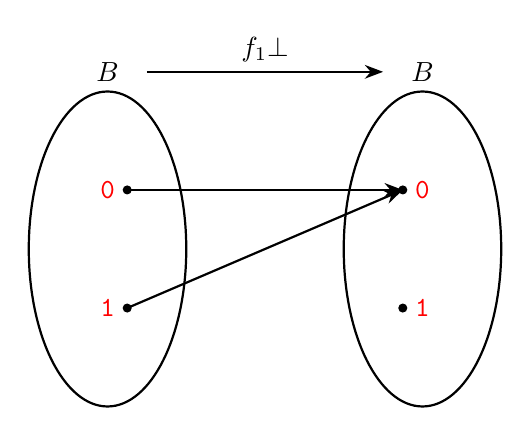
\begin{tikzpicture}
	% Draw the sets A and B
	\draw[thick] (-2,0) ellipse (1 and 2);
	\draw[thick] (2,0) ellipse (1 and 2);
	
	% Labels for sets
	\node at (-2, 2.25) {$\B$};
	\node at (2, 2.25) {$\B$};
	
	% Draw the arrows representing the function
	\draw[-Stealth, thick] (-1.5, 2.25) -- (1.5,2.25) node[midway, above] {$f_1\triangleq\bot$};
	
	\node at (-2, .75) {$\false$};
	\node at (-2, -.75) {$\true$};
	\draw[fill] (-1.75,.75) circle (.05);
	\draw[fill] (-1.75,-.75) circle (.05);
	
	\node at (2, .75) {$\false$};
	\node at (2, -.75) {$\true$};
	\draw[fill] (1.75,.75) circle (.05);
	\draw[fill] (1.75,-.75) circle (.05);
	
	\draw[-Stealth, thick] (-1.75, .75) -- (1.75, .75);
	\draw[-Stealth, thick] (-1.75, -.75) -- (1.75, .75);
\end{tikzpicture}}\\
$f_1$ is the \textit{contradiction function}.
\end{minipage}\begin{minipage}{.48\textwidth}\centering\adjustbox{scale=.9}{
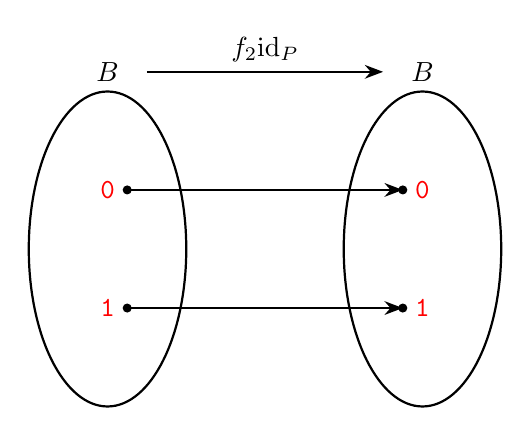
\begin{tikzpicture}
	% Draw the sets A and B
	\draw[thick] (-2,0) ellipse (1 and 2);
	\draw[thick] (2,0) ellipse (1 and 2);
	
	% Labels for sets
	\node at (-2, 2.25) {$\B$};
	\node at (2, 2.25) {$\B$};
	
	% Draw the arrows representing the function
	\draw[-Stealth, thick] (-1.5, 2.25) -- (1.5,2.25) node[midway, above] {$f_2\triangleq\id_P$};
	
	\node at (-2, .75) {$\false$};
	\node at (-2, -.75) {$\true$};
	\draw[fill] (-1.75,.75) circle (.05);
	\draw[fill] (-1.75,-.75) circle (.05);
	
	\node at (2, .75) {$\false$};
	\node at (2, -.75) {$\true$};
	\draw[fill] (1.75,.75) circle (.05);
	\draw[fill] (1.75,-.75) circle (.05);
	
	\draw[-Stealth, thick] (-1.75, .75) -- (1.75, .75);
	\draw[-Stealth, thick] (-1.75, -.75) -- (1.75, -.75);
\end{tikzpicture}}\\
$f_2$ is the \textit{identity function}
\end{minipage}
\end{center}
\begin{center}\begin{minipage}{.48\textwidth}\centering\adjustbox{scale=.9}{
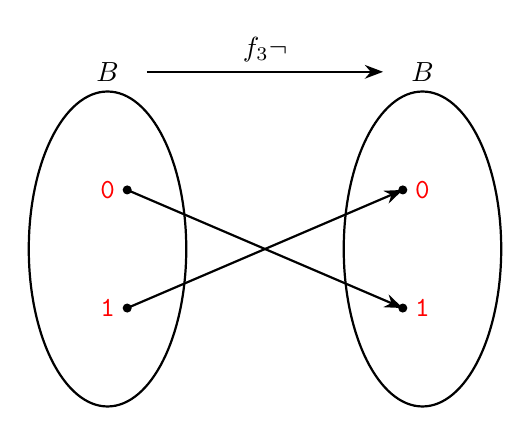
\begin{tikzpicture}
	% Draw the sets A and B
	\draw[thick] (-2,0) ellipse (1 and 2);
	\draw[thick] (2,0) ellipse (1 and 2);
	
	% Labels for sets
	\node at (-2, 2.25) {$\B$};
	\node at (2, 2.25) {$\B$};
	
	% Draw the arrows representing the function
	\draw[-Stealth, thick] (-1.5, 2.25) -- (1.5,2.25) node[midway, above] {$f_3\triangleq\lnot$};
	
	\node at (-2, .75) {$\false$};
	\node at (-2, -.75) {$\true$};
	\draw[fill] (-1.75,.75) circle (.05);
	\draw[fill] (-1.75,-.75) circle (.05);
	
	\node at (2, .75) {$\false$};
	\node at (2, -.75) {$\true$};
	\draw[fill] (1.75,.75) circle (.05);
	\draw[fill] (1.75,-.75) circle (.05);
	
	\draw[-Stealth, thick] (-1.75, .75) -- (1.75, -.75);
	\draw[-Stealth, thick] (-1.75, -.75) -- (1.75, .75);
\end{tikzpicture}}\\
$f_3$ is the \textit{logical not function}
\end{minipage}\begin{minipage}{.48\textwidth}\centering\adjustbox{scale=.9}{
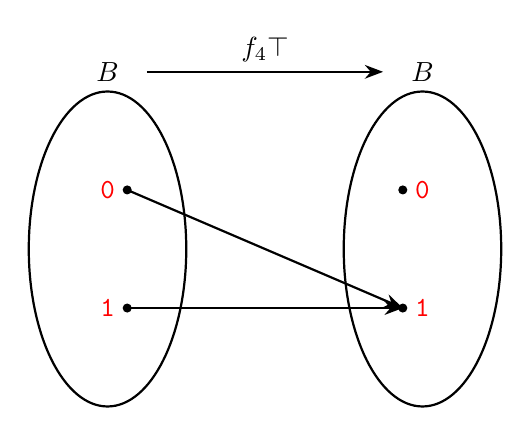
\begin{tikzpicture}
	% Draw the sets A and B
	\draw[thick] (-2,0) ellipse (1 and 2);
	\draw[thick] (2,0) ellipse (1 and 2);
	
	% Labels for sets
	\node at (-2, 2.25) {$\B$};
	\node at (2, 2.25) {$\B$};
	
	% Draw the arrows representing the function
	\draw[-Stealth, thick] (-1.5, 2.25) -- (1.5,2.25) node[midway, above] {$f_4\triangleq\top$};
	
	\node at (-2, .75) {$\false$};
	\node at (-2, -.75) {$\true$};
	\draw[fill] (-1.75,.75) circle (.05);
	\draw[fill] (-1.75,-.75) circle (.05);
	
	\node at (2, .75) {$\false$};
	\node at (2, -.75) {$\true$};
	\draw[fill] (1.75,.75) circle (.05);
	\draw[fill] (1.75,-.75) circle (.05);
	
	\draw[-Stealth, thick] (-1.75, .75) -- (1.75, -.75);
	\draw[-Stealth, thick] (-1.75, -.75) -- (1.75, -.75);
\end{tikzpicture}}\\
$f_4$ is the \textit{tautology function}
\end{minipage}
\end{center}
\end{proof}

\newpage
\begin{remark}[Group Structure]
\ \begin{itemize}
	\item $\left(\set{\id_P,\lnot},\circ\right)$ is a group, but $\left(\set{\id_P,\bot},\circ\right)$ and $\left(\set{\id_P,\top},\circ\right)$ are not: \begin{table}[h!]\centering
	\begin{tabular}{c|cc}
		\hline
		$\circ$ & $\id_P$ & $\lnot$ \\ \hline
		$\id_P$ & $\id_P$ & $\lnot$ \\
		$\lnot$ & $\lnot$ & $\id_P$ \\ \hline
	\end{tabular}\quad\quad
	\begin{tabular}{c|cc}
		\hline
		$\circ$ & $\id_P$ & $\bot$ \\ \hline
		$\id_P$ & $\id_P$ & $\bot$ \\
		$\bot$ & $\bot$ & $\bot$ \\ \hline
	\end{tabular}\quad\quad
	\begin{tabular}{c|cc}
		\hline
		$\circ$ & $\id_P$ & $\top$ \\ \hline
		$\id_P$ & $\id_P$ & $\top$ \\
		$\top$ & $\top$ & $\top$ \\ \hline
	\end{tabular}
	\end{table}
\end{itemize}	
\end{remark}

\begin{remark}
The structure is a non-associative magma, also known as a groupoid. \begin{table}[h!]\centering
	\begin{tabular}{c||c|c|c|c}
		$\circ$ & $\bot$ & $P$ & $\lnot$ & $\top$ \\ \hline\hline
		$\bot$ & $\bot$ & $\bot$ & $\top$ & $\top$ \\ \hline
		$P$ & $\bot$ & $P$ & $\lnot$ & $\top$ \\ \hline
		$\lnot$ & $\bot$ & $\lnot$ & $P$ & $\top$ \\ \hline
		$\top$ & $\bot$ & $\top$ & $\bot$ & $\top$
	\end{tabular}
\end{table}
\end{remark}

\begin{tcolorbox}[colframe=corcolor,title={\color{white}\bf Binary Truth Functions}]
	\begin{corollary}
		There are 16 distinct binary truth functions:
		\begin{itemize}
			\item Two \textit{constant operations}:
			\begin{itemize}
				\item $f_{\true}(p,q)=\true$
				\item $f_{\false}(p,q)=\false$
			\end{itemize}
			\item Two \textit{projections}:
			\begin{itemize}
				\item $\mathsf{Proj}_1(p,q)=p$
				\item $\mathsf{Proj}_2(p,q)=q$
			\end{itemize} 
			\item Two \textit{negated projections}:
			\begin{itemize}
				\item $\overline{\mathsf{Proj}_1}(p,q)=\lnot p$
				\item $\overline{\mathsf{Proj}_2}(p,q)=\lnot q$
			\end{itemize} 
			\item The \textit{conjunction}: $p\land q$
			\item The \textit{disjunction}: $p\lor q$
			\item Two \textit{conditionals}:
			\begin{itemize}
				\item $p\implies q$
				\item $q\implies p$
			\end{itemize}
			\item The \textit{biconditional} (iff): $p\iff q$
			\item The \textit{exclusive or} (xor): $\lnot(p\iff q)$
			\item Two \textit{negated conditionals}:
			\begin{itemize}
				\item $\lnot(p\implies q)$
				\item $\lnot(q\implies p)$
			\end{itemize}
			\item The \textit{NAND} $p\uparrow q$
			\item The \textit{NOR} $p\downarrow q$
		\end{itemize}
	\end{corollary}
\end{tcolorbox}
\begin{proof}
	From Count of Truth Functions there are $2^{(2^2)}=16$
	distinct truth functions on 2 variable. These can be depicted in a truth table as follows:
	\begin{table}[h!]\centering
		\begin{tabular}{|r|cccc|}
			\hline
			$p$ & $\true$ & $\true$ & $\false$ & $\false$ \\
			$q$ & $\true$ & $\false$ & $\true$ & $\false$ \\
			\hline
			$f_{\false}(p,q)$ & $\false$ & $\false$ & $\false$ & $\false$ \\
			$p\downarrow q$ & $\false$ & $\false$ & $\false$ & $\true$ \\
			$\lnot(p\impliedby q)$ & $\false$ & $\false$ & $\true$ & $\false$ \\
			$\overline{\mathsf{Proj}_1}(p,q)$ & $\false$ & $\false$ & $\true$ & $\true$ \\
			$\lnot(p\implies q)$ & $\false$ & $\true$ & $\false$ & $\false$ \\
			$\overline{\mathsf{Proj}_2}(p,q)$ & $\false$ & $\true$ & $\false$ & $\true$ \\
			$\lnot(p\iff q)$ & $\false$ & $\true$ & $\true$ & $\false$ \\
			$p\uparrow q$ & $\false$ & $\true$ & $\true$ & $\true$ \\
			$p\land q$ & $\true$ & $\false$ & $\false$ & $\false$ \\
			$p\iff q$ & $\true$ & $\false$ & $\false$ & $\true$ \\
			$\mathsf{Proj}_2(p,q)$ & $\true$ & $\false$ & $\true$ & $\false$ \\
			$p\implies q$ & $\true$ & $\false$ & $\true$ & $\true$ \\
			$\mathsf{Proj}_1(p,q)$ & $\true$ & $\true$ & $\false$ & $\false$ \\
			$p\impliedby q$ & $\true$ & $\true$ & $\false$ & $\true$ \\
			$p\lor q$ & $\true$ & $\true$ & $\true$ & $\false$ \\
			$f_{\true}(p,q)$ & $\true$ & $\true$ & $\true$ & $\true$ \\
			\hline
		\end{tabular}
	\end{table}
	\begin{center}\begin{minipage}{.48\textwidth}\centering\adjustbox{scale=.9}{
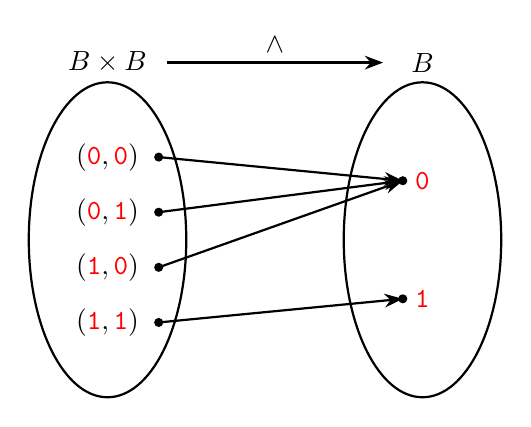
\begin{tikzpicture}
	% Draw the sets A and B
	\draw[thick] (-2,0) ellipse (1 and 2);
	\draw[thick] ( 2,0) ellipse (1 and 2);
	
	% Labels for sets
	\node at (-2, 2.25) {$\B\times\B$};
	\node at ( 2, 2.25) {$\B$};
	
	% Draw the arrows representing the function
	\draw[-Stealth, thick] (-1.25, 2.25) -- (1.5,2.25) node[midway, above] {$\land$};
	
	\node at (-2,  1.05) {$(\false,\false)$};
	\node at (-2,   .35) {$(\false,\true)$};
	\node at (-2, - .35) {$(\true,\false)$};
	\node at (-2, -1.05) {$(\true,\true)$};
	\draw[fill] (-1.35, 1.05) circle (.05);
	\draw[fill] (-1.35,  .35) circle (.05);
	\draw[fill] (-1.35, -.35) circle (.05);
	\draw[fill] (-1.35,-1.05) circle (.05);
	
	\node at (2,  .75) {$\false$};
	\node at (2, -.75) {$\true$};
	\draw[fill] (1.75, .75) circle (.05);
	\draw[fill] (1.75,-.75) circle (.05);
	
	\draw[-Stealth, thick] (-1.35, 1.05) -- (1.75, .75);
	\draw[-Stealth, thick] (-1.35, .35) -- (1.75, .75);
	\draw[-Stealth, thick] (-1.35, -.35) -- (1.75, .75);
	\draw[-Stealth, thick] (-1.35, -1.05) -- (1.75, -.75);
\end{tikzpicture}}\\
\end{minipage}\begin{minipage}{.48\textwidth}\centering\adjustbox{scale=.9}{
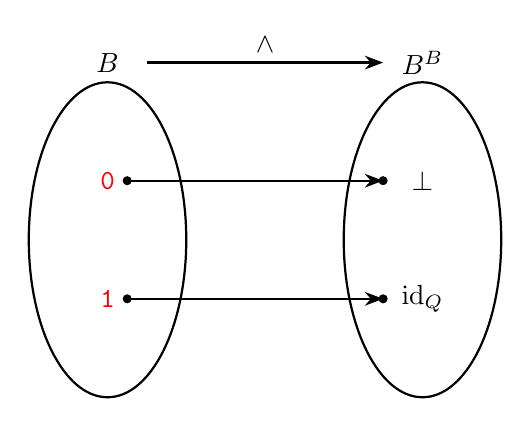
\begin{tikzpicture}
	% Draw the sets A and B
	\draw[thick] (-2,0) ellipse (1 and 2);
	\draw[thick] ( 2,0) ellipse (1 and 2);
	
	% Labels for sets
	\node at (-2, 2.25) {$\B$};
	\node at ( 2, 2.25) {$\B^{\B}$};
	
	% Draw the arrows representing the function
	\draw[-Stealth, thick] (-1.5, 2.25) -- (1.5,2.25) node[midway, above] {$\land$};
	
	\node at (-2, .75) {$\false$};
	\node at (-2, -.75) {$\true$};
	\draw[fill] (-1.75,.75) circle (.05);
	\draw[fill] (-1.75,-.75) circle (.05);
	
	\node at (2, .75) {$\bot$};
	\node at (2, -.75) {$\id_Q$};
	\draw[fill] (1.5,.75) circle (.05);
	\draw[fill] (1.5,-.75) circle (.05);
	
	\draw[-Stealth, thick] (-1.75, .75) -- (1.5, .75);
	\draw[-Stealth, thick] (-1.75, -.75) -- (1.5, -.75);
\end{tikzpicture}}\\
\end{minipage}\end{center}

\begin{center}\begin{minipage}{.48\textwidth}\centering\adjustbox{scale=.9}{
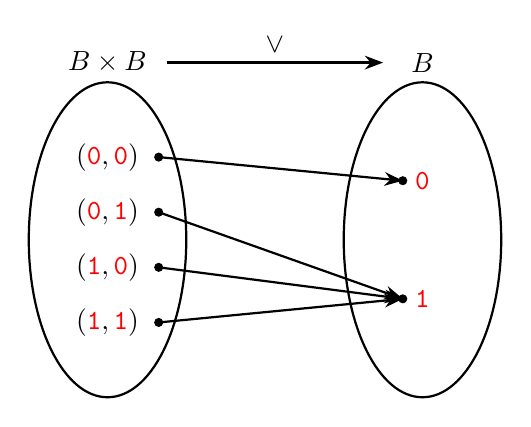
\begin{tikzpicture}
	% Draw the sets A and B
	\draw[thick] (-2,0) ellipse (1 and 2);
	\draw[thick] ( 2,0) ellipse (1 and 2);
	
	% Labels for sets
	\node at (-2, 2.25) {$\B\times\B$};
	\node at ( 2, 2.25) {$\B$};
	
	% Draw the arrows representing the function
	\draw[-Stealth, thick] (-1.25, 2.25) -- (1.5,2.25) node[midway, above] {$\lor$};
	
	\node at (-2,  1.05) {$(\false,\false)$};
	\node at (-2,   .35) {$(\false,\true)$};
	\node at (-2, - .35) {$(\true,\false)$};
	\node at (-2, -1.05) {$(\true,\true)$};
	\draw[fill] (-1.35, 1.05) circle (.05);
	\draw[fill] (-1.35,  .35) circle (.05);
	\draw[fill] (-1.35, -.35) circle (.05);
	\draw[fill] (-1.35,-1.05) circle (.05);
	
	\node at (2,  .75) {$\false$};
	\node at (2, -.75) {$\true$};
	\draw[fill] (1.75, .75) circle (.05);
	\draw[fill] (1.75,-.75) circle (.05);
	
	\draw[-Stealth, thick] (-1.35, 1.05) -- (1.75, .75);
	\draw[-Stealth, thick] (-1.35, .35) -- (1.75, -.75);
	\draw[-Stealth, thick] (-1.35, -.35) -- (1.75, -.75);
	\draw[-Stealth, thick] (-1.35, -1.05) -- (1.75, -.75);
\end{tikzpicture}}\\
\end{minipage}\begin{minipage}{.48\textwidth}\centering\adjustbox{scale=.9}{
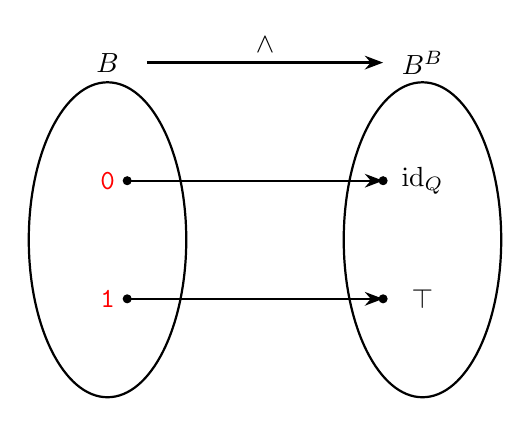
\begin{tikzpicture}
	% Draw the sets A and B
	\draw[thick] (-2,0) ellipse (1 and 2);
	\draw[thick] ( 2,0) ellipse (1 and 2);
	
	% Labels for sets
	\node at (-2, 2.25) {$\B$};
	\node at ( 2, 2.25) {$\B^{\B}$};
	
	% Draw the arrows representing the function
	\draw[-Stealth, thick] (-1.5, 2.25) -- (1.5,2.25) node[midway, above] {$\land$};
	
	\node at (-2, .75) {$\false$};
	\node at (-2, -.75) {$\true$};
	\draw[fill] (-1.75,.75) circle (.05);
	\draw[fill] (-1.75,-.75) circle (.05);
	
	\node at (2, .75) {$\id_Q$};
	\node at (2, -.75) {$\top$};
	\draw[fill] (1.5,.75) circle (.05);
	\draw[fill] (1.5,-.75) circle (.05);
	
	\draw[-Stealth, thick] (-1.75, .75) -- (1.5, .75);
	\draw[-Stealth, thick] (-1.75, -.75) -- (1.5, -.75);
\end{tikzpicture}}\\
\end{minipage}\end{center}

\begin{center}\begin{minipage}{.48\textwidth}\centering\adjustbox{scale=.9}{
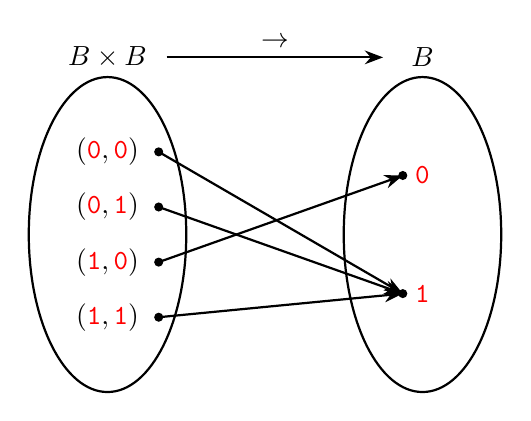
\begin{tikzpicture}
	% Draw the sets A and B
	\draw[thick] (-2,0) ellipse (1 and 2);
	\draw[thick] ( 2,0) ellipse (1 and 2);
	
	% Labels for sets
	\node at (-2, 2.25) {$\B\times\B$};
	\node at ( 2, 2.25) {$\B$};
	
	% Draw the arrows representing the function
	\draw[-Stealth, thick] (-1.25, 2.25) -- (1.5,2.25) node[midway, above] {$\to$};
	
	\node at (-2,  1.05) {$(\false,\false)$};
	\node at (-2,   .35) {$(\false,\true)$};
	\node at (-2, - .35) {$(\true,\false)$};
	\node at (-2, -1.05) {$(\true,\true)$};
	\draw[fill] (-1.35, 1.05) circle (.05);
	\draw[fill] (-1.35,  .35) circle (.05);
	\draw[fill] (-1.35, -.35) circle (.05);
	\draw[fill] (-1.35,-1.05) circle (.05);
	
	\node at (2,  .75) {$\false$};
	\node at (2, -.75) {$\true$};
	\draw[fill] (1.75, .75) circle (.05);
	\draw[fill] (1.75,-.75) circle (.05);
	
	\draw[-Stealth, thick] (-1.35, 1.05) -- (1.75, -.75);
	\draw[-Stealth, thick] (-1.35, .35) -- (1.75, -.75);
	\draw[-Stealth, thick] (-1.35, -.35) -- (1.75, .75);
	\draw[-Stealth, thick] (-1.35, -1.05) -- (1.75, -.75);
\end{tikzpicture}}\\
\end{minipage}\begin{minipage}{.48\textwidth}\centering\adjustbox{scale=.9}{
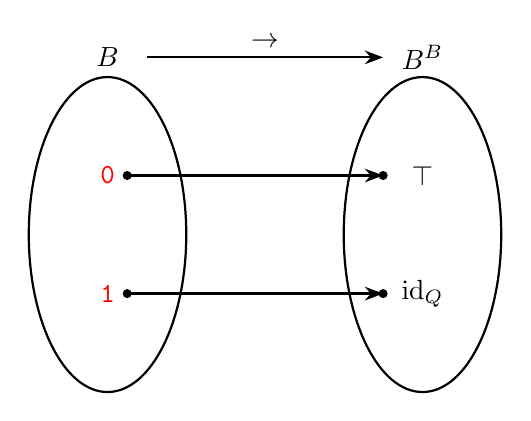
\begin{tikzpicture}
	% Draw the sets A and B
	\draw[thick] (-2,0) ellipse (1 and 2);
	\draw[thick] ( 2,0) ellipse (1 and 2);
	
	% Labels for sets
	\node at (-2, 2.25) {$\B$};
	\node at ( 2, 2.25) {$\B^{\B}$};
	
	% Draw the arrows representing the function
	\draw[-Stealth, thick] (-1.5, 2.25) -- (1.5,2.25) node[midway, above] {$\to$};
	
	\node at (-2, .75) {$\false$};
	\node at (-2, -.75) {$\true$};
	\draw[fill] (-1.75,.75) circle (.05);
	\draw[fill] (-1.75,-.75) circle (.05);
	
	\node at (2, .75) {$\top$};
	\node at (2, -.75) {$\id_Q$};
	\draw[fill] (1.5,.75) circle (.05);
	\draw[fill] (1.5,-.75) circle (.05);
	
	\draw[-Stealth, thick] (-1.75, .75) -- (1.5, .75);
	\draw[-Stealth, thick] (-1.75, -.75) -- (1.5, -.75);
\end{tikzpicture}}\\
\end{minipage}\end{center}

\begin{center}\begin{minipage}{.48\textwidth}\centering\adjustbox{scale=.9}{
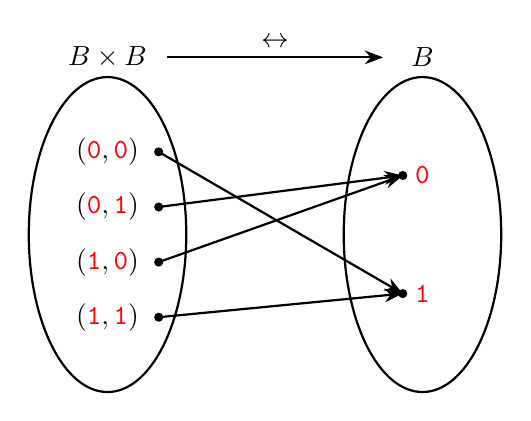
\begin{tikzpicture}
	% Draw the sets A and B
	\draw[thick] (-2,0) ellipse (1 and 2);
	\draw[thick] ( 2,0) ellipse (1 and 2);
	
	% Labels for sets
	\node at (-2, 2.25) {$\B\times\B$};
	\node at ( 2, 2.25) {$\B$};
	
	% Draw the arrows representing the function
	\draw[-Stealth, thick] (-1.25, 2.25) -- (1.5,2.25) node[midway, above] {$\leftrightarrow$};
	
	\node at (-2,  1.05) {$(\false,\false)$};
	\node at (-2,   .35) {$(\false,\true)$};
	\node at (-2, - .35) {$(\true,\false)$};
	\node at (-2, -1.05) {$(\true,\true)$};
	\draw[fill] (-1.35, 1.05) circle (.05);
	\draw[fill] (-1.35,  .35) circle (.05);
	\draw[fill] (-1.35, -.35) circle (.05);
	\draw[fill] (-1.35,-1.05) circle (.05);
	
	\node at (2,  .75) {$\false$};
	\node at (2, -.75) {$\true$};
	\draw[fill] (1.75, .75) circle (.05);
	\draw[fill] (1.75,-.75) circle (.05);
	
	\draw[-Stealth, thick] (-1.35, 1.05) -- (1.75, -.75);
	\draw[-Stealth, thick] (-1.35, .35) -- (1.75, .75);
	\draw[-Stealth, thick] (-1.35, -.35) -- (1.75, .75);
	\draw[-Stealth, thick] (-1.35, -1.05) -- (1.75, -.75);
\end{tikzpicture}}\\
\end{minipage}\begin{minipage}{.48\textwidth}\centering\adjustbox{scale=.9}{
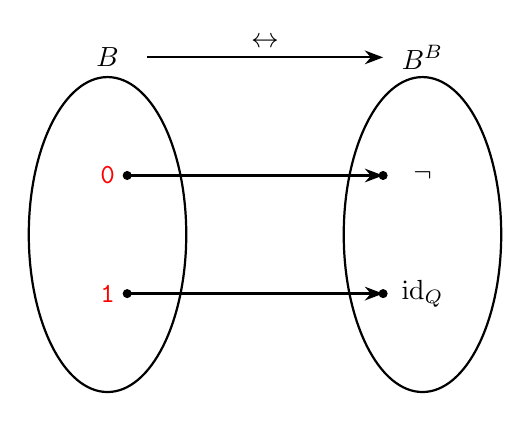
\begin{tikzpicture}
	% Draw the sets A and B
	\draw[thick] (-2,0) ellipse (1 and 2);
	\draw[thick] ( 2,0) ellipse (1 and 2);
	
	% Labels for sets
	\node at (-2, 2.25) {$\B$};
	\node at ( 2, 2.25) {$\B^{\B}$};
	
	% Draw the arrows representing the function
	\draw[-Stealth, thick] (-1.5, 2.25) -- (1.5,2.25) node[midway, above] {$\leftrightarrow$};
	
	\node at (-2, .75) {$\false$};
	\node at (-2, -.75) {$\true$};
	\draw[fill] (-1.75,.75) circle (.05);
	\draw[fill] (-1.75,-.75) circle (.05);
	
	\node at (2, .75) {$\lnot$};
	\node at (2, -.75) {$\id_Q$};
	\draw[fill] (1.5,.75) circle (.05);
	\draw[fill] (1.5,-.75) circle (.05);
	
	\draw[-Stealth, thick] (-1.75, .75) -- (1.5, .75);
	\draw[-Stealth, thick] (-1.75, -.75) -- (1.5, -.75);
\end{tikzpicture}}\\
\end{minipage}\end{center}
\end{proof}


\newpage
%\begin{tcolorbox}[colframe=defcolor,title={\color{white}\bf Formal Grammer}]
%	\begin{definition}
%		The formal grammar of the language of propositional logic (and hence its WFFs) can be defined in the following ways.
%		\begin{itemize}
%			\item \textbf{Backus-Naur Form}
%			In Backus-Naur form, the formal grammar of the language of propositional logic takes the following form:
%			\begin{align*}
%				<\texttt{formula}>\quad &::=\quad p\mid\top\mid\bot &\text{where $p\in\mathcal{P}_0$ is a letter}\\
%				<\texttt{formula}>\quad &::=\quad \lnot<\texttt{formula}>\\
%				<\texttt{formula}>\quad &::=\quad (<\texttt{formula}> <\texttt{op}> <\texttt{formula}>)\\
%				<\texttt{op}>\quad &::=\quad \land\mid\lor\mid\implies\mid\iff
%			\end{align*} Note that this is a top-down grammar:
%			we start with a metasymbol <formula>
%			progressively replace it with constructs containing other metasymbols and/or primitive symbols
%			until finally we are left with a well-formed formula of L0
%			consisting of nothing but primitive symbols.
%		\end{itemize}
%		
%	\end{definition}
%\end{tcolorbox}

\section{Backus-Naur Form (BNF)}

Backus-Naur Form (BNF) is a notation technique for context-free grammars, often used to describe the syntax of languages used in computing. Introduced by John Backus and Peter Naur in the 1960s, BNF was initially developed to describe the syntax of the ALGOL 60 programming language.

A grammar defines a language by providing a set of production rules that describe how sentences in the language can be formed. BNF uses non-terminal symbols, terminal symbols, and production rules to define these grammars.

Non-terminal symbols are placeholders for patterns of terminal symbols that can be generated by applying production rules.

Terminal symbols are the actual symbols of the language's alphabet, and they appear in the strings generated by the grammar.

Production rules define how non-terminal symbols can be replaced with combinations of non-terminal and terminal symbols. BNF uses a specific syntax to describe these rules:

\begin{verbatim}
	<rule-name> ::= <expression>
\end{verbatim}

Extended BNF (EBNF) provides additional notation to simplify grammar definitions, such as optional elements and repetitions.

BNF is a powerful tool for defining the syntax of programming languages and has been fundamental in the development of many language specifications. For more information, refer to resources such as the \emph{ALGOL 60 Report}, or textbooks on formal language theory and compiler design.


\begin{example}
Here is an example of BNF describing simple arithmetic expressions:
\begin{verbatim}
	<expression> ::= <term> | <term> "+" <expression>
	<term> ::= <factor> | <factor> "*" <term>
	<factor> ::= <number> | "(" <expression> ")"
	<number> ::= "0" | "1" | "2" | "3" | "4" | "5" | "6" | "7" | "8" | "9"
\end{verbatim}
\end{example}




	
%	\footnotesize
	\bibliographystyle{plain}
%	\bibliographystyle{plainnat}  % Use the plainnat style
	\bibliography{sv-references}
	
\end{document}
